\documentclass[12pt,draftclsnofoot,onecolumn,journal]{IEEEtran}
%\documentclass[transmag]{IEEEtran}
\usepackage{latexsym}
\usepackage{graphicx}
\usepackage{amsfonts,amssymb,amsmath,cite}
\usepackage[colorlinks=true,linkcolor=black,anchorcolor=black,citecolor=black,filecolor=black,menucolor=black,runcolor=black,urlcolor=black]{hyperref}
\usepackage{bbm}
\usepackage{paralist}
\usepackage{algpseudocode}
\usepackage[nolist]{acronym}
%\usepackage{algorithmicx}
\usepackage{algorithm}
\usepackage[dvipsnames]{xcolor}
\usepackage{amsthm}
\usepackage{amsmath}
\usepackage{microtype}
\usepackage{algpseudocode}
\usepackage{algorithm}
\usepackage{tabularx}
\usepackage{bbm}
\usepackage{pdfpages}
\usepackage{amsthm}
\usepackage{amsmath}

\usepackage{subfig}
\usepackage{graphicx}

%% Define Macros! That makes life much easier 
\newtheorem{theorem}{Theorem}
\newcommand{\cmt}[1]{\textcolor{red}{#1} }
\newcommand{\brc}[1]{ \left( #1 \right) }
\newcommand{\dbc}[1]{ \left[ #1 \right] }
\newcommand{\Diag}[1]{ \mathrm{Diag}\left\lbrace #1 \right\rbrace }
\newcommand{\e}{\mathrm{e}}
\newcommand{\trp}{\mathsf{T}}

\newcommand{\Ex}[1]{ \mathbbmss{E}\left\lbrace #1 \right\rbrace }
\newcommand{\norm}[1]{ \left\Vert #1 \right\Vert}
\newcommand{\abs}[1]{ \left\vert #1 \right\vert}



\begin{document}

\title{ HYBRID ANALOG-DIGITAL TRANSMITTER WITH PASSIVE ANTENNA ARRAY}

\author{Zilu Zhao, Ali Bereyhi
\thanks{
Author is with IDC, FAU.
}
}

\IEEEoverridecommandlockouts
\maketitle

\section{Introduction}
Millimeter-wave communication is one of the technologies that enable the high-bandwidth communication. However, due to the small wave length, antenna arrays are often required to compensate for the high loss, which will increase the hardware complexity. In article \cite{alkhateeb2014mimo}, two methods are investigated, low-resolution ADCs and \ac{had} precoding. Receivers equipped low-resolution ADCs have low power consumption but require more RF chains. On the contrary, systems employing \ac{had} architecture requires less RF chains than the antenna amount, but the performance is limited by the number of RF chains. Low complexity algorithms have also been developed for the \ac{had} systems such as SIC-based hybrid precoding \cite{gao2016energy}. This precoding method avoid the SVD operations and is more energy efficient than the fully digital systems.

\Ac{irs} is a newly proposed reconfigurable communication component \cite{wu2021intelligent}. It contains a large number of passive antenna elements whose amplitude/phase is adjustable. Typical applications of \ac{irs} includes creating a virtual line-of-sight, providing extra flexibility in resource allocation and so on \cite{wu2019towards}.  When the \ac{irs} used as a relay, some alternating algorithm can be used with semidefinite relaxation to offer a trade-off between performance and computational complexity \cite{wu2019intelligent}. It is also shown in \cite{wu2019intelligent} that the use of \ac{irs} is more cost efficient than conventional amplify-and-forward relay. For the purpose of resource allocation, \ac{irs} can be employed to degrade the channel quality of eavesdroppers \cite{xu2019resource} to enhance the physical layer security. In \cite{xu2022optimal}, algorithms for providing energy for the energy hungry units while keeping the quality of service for the information decoding receivers with \ac{irs} structures are provided.

Beside being used as a passive relay, the \ac{irs} can also be utilized as a passive unit of the \ac{bs}. In this scenario, one or multiple RF chains are placed in the close proximity of the \ac{irs} serving as energy feeder or data feeder. With even only one RF chain, a variate of usages can be achieved by such \ac{irs}-aided transmitter structure. For example, \ac{irs}-based modulation, \ac{irs}-based transmitter and \ac{irs}-based encoding \cite{di2020smart}. The idea of spatial modulation is to embed the information in both the choice of the constellation symbols and the choice of the antenna indeces \cite{di2011spatial}. Besides turning certain \ac{irs} regions on and off \cite{di2020smart}, two other index modulation methods are studied in \cite{basar2020reconfigurable} for receiver antennas, which are \ac{irs}-space shift keying and \ac{irs}-spatial modulation. The \ac{irs}-space shift keying method root the information purely into the selection of antenna index while \ac{irs}-spatial modulation embeds partial information also into the transmitted signal of the RF chain. By using this structure as an \ac{irs}-based transmitter, the \ac{irs} is only fed with carrier signals by the RF chain. Such application is investigated in \cite{liu2021intelligent} and a symbol wise precoding method is adopted to design the \ac{irs} configurations. Some analytical investigations for the single-RF chain \ac{irs}-based transmission systems are conducted in \cite{karasik2020beyond}, and states that joint encoding of the RF chain and the \ac{irs} is necessary to achieve max rate. The \ac{irs}-aided hybrid 
transmitters use a digital unit connected to multiple RF chains and an \ac{irs} as the analog unit. In \cite{jamali2020intelligent}, point to point \ac{mimo} communication employing such \ac{irs}-aided hybrid transmission structure is studied, and two block-level precoding methods depending only on \ac{csi} are proposed. Multi-user scenario is investigated in \cite{bereyhi2019papr}, which transforms the precoding task into a \ac{glse} problem to make both average power and peak power controllable.

The precoding methods can be generally divided into two categories, which are block level precoding and symbol level precoding \cite{domouchtsidis2020constant}. In conventional block level precoding, the transmitter utilize the \ac{csi} without the knowledge of the data messages. However, in symbol level precoding, both \ac{csi} and knowledge of the data messages are taken into considerations to generate the precoding symbols. As is discussed above two convensional block level precoding method for \ac{irs}-aided hybrid transmission systems are discussed in \cite{jamali2020intelligent}, which are based on maximizing the mutual information and approximating the optimal fully digital precoder. The advantage of the block level precoding is low computational complexity and low update rate at the \ac{irs} unit. The analog units are often designed on block level because of practical reason \cite{li2018hybrid}, but symbol level precoding methods based on both \ac{csi} and information messages can be designed for digital units. Symbol level precoding introduced in \cite{liu2019symbol} exploit the constructive interference in modulated communication to push the received signal away from decision boundary and hence increase the performance. The article \cite{li2022practical} utilizes the idea of constructive interference with block level precoding and employs such method in a conventional \ac{mimo} system. In this article, we wish to calculate the precoded symbols for the digital outputs and \ac{irs} configurations in one block jointly. In other words, we want to designed digital unit and the \ac{irs} based on the knowledge of both the \ac{csi} and information messages. Furthermore, Gaussian signaling is used. In a fully connected hybrid analog digital precoder, an alternating algorithm is suggested in \cite{sedaghat2017novel}, and some theoretical results about the block length and RF chain amount are also given.

This article investigates the precoding scheme in \ac{irs} aided \ac{had} systems. The precoding task cannot be formulated as a convex problem. Hence, alternating optimization method is used to optimize the digital unit outputs and \ac{irs} configurations. In the meantime, we find out that the optimization of the digital unit output is a convex problem, while the optimization of the \ac{irs} configurations is non-convex. We use gradient descent and \ac{mm} algorithm to reconfigure the \ac{irs}. Since the passive antenna elements on the \ac{irs} are relative cheap, this article also studies the relation between \ac{irs} size and block length. \\
\textbf{Notation}:
The $\delta(\cdot)$ is the discrete Dirac function which is evaluated to zero when it has non-zero argument and evaluate to one when its argument is zero.



\section{Problem Formulation}
%\subsection{System Model}
Consider downlink transmission in a multi-user \ac{mimo} system where a \ac{bs} equipped with $M$ antenna elements simultaneously serves $K$ single-antenna \acp{ut}. The \ac{bs} employs an \ac{irs}-aided \ac{had} architecture whose digital unit contains $N$ \ac{rf}-chains and whose analog unit is realized via a passive \ac{irs} with $M$ reflecting elements.%; see Fig. \ref{fig:sysmodel_illustration}. 

%The transmitter intends to send information symbols $s_{k,n}$ to \ac{ut} $k$ in symbol interval $\ell$ for $k\in \dbc{K}$ and $n\in\dbc{N}$. To this end, it groups the symbols of the \acp{ut} into blocks of length $L$ for some $L$. 
%\begin{equation}
%\mathbf S =\left[ \mathbf s_1, \mathbf s_2, \ldots,  \mathbf s_L \right]
%\end{equation}
%and then
%
%At time interval $\ell$ drawn from one time block, we denote the coded information symbols to be transmitted as $\mathbf{s}_n=\left[ s_1, s_2, \cdots, s_K \right]^{\mathsf{T}}$. Matrix 

% is used to represent all information message symbols in one time block. 
\subsection{Transmitter Architecture}
The architecture of the transmitter is depicted in Fig.~\ref{fig:sysmodel_illustration}. The digital unit is modeled as a generic non-linear function $\Pi_\ell\brc{\cdot}: \mathbb C^{K} \mapsto \mathbb C^{M}$, which determines the precoded signals in the base-band digital domain based on both information symbols and \ac{csi}. The digitally-precoded signal in the symbol interval $\ell$, i.e., $\mathbf{x}_\ell \in \mathbb{C}^N$, can hence be written as 
\begin{align}
\mathbf x_\ell = \Pi_\ell\brc{ \mathbf s_\ell  \vert \mathbf H},
\end{align}
and is assumed to satisfy 
\begin{align}
	\Ex{ \norm{\mathbf x_\ell}^2 } \leq P_{\rm avg}
\end{align}
for some average transmit power $P_{\rm avg}$. To avoid nonlinear distortion at the \ac{rf}-chains, the digital unit further restricts the peak instantaneous power of the signal, i.e., at any given time interval $\ell$,
\begin{align}
\abs{x_{k,\ell}}^2 \leq P_{\max}
\end{align}
for $k\in\dbc{K}$ and some peak power $P_{\max}$.


At the output of the digital unit, the signal $\mathbf{x}_\ell$ is up-converted to the \ac{rf} domain and illuminated via the \ac{rf}-chains towards the \ac{irs}. Since the digital and \ac{irs} unit are located closely, the illumination channel between them can be regarded as a noise-free linear transform whose transfer matrix is  $\mathbf T\in\mathbb C^{M\times N}$ is given by \cite{jamali2020intelligent}
\begin{equation}
\mathbf T=\begin{bmatrix}
\frac{\lambda_{\mathrm w}\sqrt{\rho G^{\mathrm a}(\theta^{\mathrm p}_{m,n}, \phi^{\mathrm p}_{m,n})G^{\mathrm p}(\theta^{\mathrm a}_{m,n}, \phi^{\mathrm a}_{m,n})}}{4\pi r_{m,n}}e^{-j\frac{2\pi r_{m,n}}{\lambda_{\mathrm w}}}
\end{bmatrix}_{m,n},
\label{eq:illuminationbasic}
\end{equation}
where $\lambda_w$ is the wavelength,  $\rho\in[0,1]$ denotes the power efficiency of the \ac{irs}. The function $G^{\mathrm a}(\theta^{\mathrm p}_{m,n}, \phi^{\mathrm p}_{m,n})$ and $G^{\mathrm p}(\theta^{\mathrm a}_{m,n}, \phi^{\mathrm a}_{m,n})$ model the antenna gain of the active antenna and the \ac{irs} element respectively. The variable $r_{m,n}$ measures the distance from the $m$-th IRS element to the $n$-th active antenna.


We assume here that the IRS elements reflect all the signals in front of them, therefore we have 
\begin{equation}
G^{\mathrm p}(\theta, \phi)=\begin{cases}
2 & \theta, \phi\in[0,\pi] \\
0 & \, \text{otherwise}
\end{cases}.
\end{equation}

The active antenna gain following \cite{jamali2020intelligent} is assumed to be 
\begin{equation}
G^{\mathrm a}(\theta, \phi)=\begin{cases}
2(1+\kappa)\cos^\kappa(\phi) & \phi\in[0,\pi/2] \\
0 & \, \text{otherwise}
\end{cases}.
\end{equation}
The $\kappa$ here is a normalization factor which ensures that the spherical surface integral of $G^{\mathrm a}(\theta, \phi)$ is $4\pi$. With larger $\kappa$, the beam from the active antenna will be more concentrated to its main direction.


At the symbol interval $\ell$, the \ac{irs} receives the signal $\mathbf{r}_\ell \in \mathbb C^{M}$ which is given by
\begin{align}
	\mathbf{r}_\ell = \mathbf{T} \mathbf{x}_\ell.
\end{align}
Each reflecting element on the  \ac{irs} reflects its received signal, i.e., $r_{m,\ell}$ for $m\in \dbc{1, M}$, with an adjustable phase-shift. As a result, the output signal of the transmitter, i.e., the signal reflected by the \ac{irs}, in the symbol interval $\ell$ is given by
\begin{align}
	\mathbf{z}_\ell = \mathbf{A}_\ell \mathbf{r}_\ell
\end{align}
where $\mathbf{A}_\ell = \Diag{ \e^{j\beta_{1,\ell}} , \ldots, \e^{j\beta_{M,\ell}} }$ with $\beta_{m,\ell}$ denoting the phase-shift applied by the reflecting element $m$ in interval $\ell$.
%\begin{equation}
%\mathbf A=
%\begin{bmatrix}
%e^{j\beta_1} & & \\
%&\ddots &\\
%& & e^{j\beta_M}
%\end{bmatrix}\in\mathbb C^{M\times M}.
%\end{equation}

\subsection{Downlink Transmission and CSI Acquisition}
The signal received by \ac{ut} $k$ in symbol interval $\ell$ is given by
\begin{equation}
y_{k,\ell} =\mathbf{h}_{k,\ell}^{\mathsf{T}} \mathbf{z}_\ell+ w_{k,\ell},
\end{equation}
where $\mathbf{h}_{k, \ell} \in \mathbb{C}^{M}$ denotes the vector of downlink channel coefficients from the \ac{bs} to the $k$-th \ac{ut}, and $w_{k,\ell}$ is \ac{AWGN} with variance $\sigma^2$, i.e., $w_{k,\ell}\sim\mathcal{CN} \brc{ 0, \sigma^2}$. Considering the transmitter architecture, the vector of received signals at the \acp{ut}, i.e., $\mathbf{y}_\ell = \dbc{y_{1,\ell}, \ldots, y_{K,\ell}}^{\mathsf T}$, is compactly represented in terms of the digitally-precoded signal $\mathbf{x}_\ell$ as
\begin{equation}
\mathbf{y}_{\ell} =\mathbf{H}_\ell^\trp \mathbf A_\ell \mathbf T \mathbf{x}_\ell + \mathbf{w}_{\ell}
\end{equation}
where the matrix $\mathbf{H}_\ell \in \mathbb{C}^{M\times K}$ is given by
\begin{align}
	\mathbf{H}_\ell = \dbc{ \mathbf{h}_{1,\ell} , \ldots, \mathbf{h}_{K,\ell} }
\end{align}
and denotes the channel matrix between the \ac{bs} to \acp{ut}. Moreover, the vector $\mathbf{w}_{n} = \dbc{w_{1,\ell}, \ldots, w_{K,\ell}}$ collects the samples of the \ac{AWGN} processes in symbol interval $\ell$. 

The system is assumed to perform in the \ac{tdd} mode. This means that uplink and downlink transmissions are divided in time domain, and hence the uplink and downlink channels are reciprocal. Using this property, the \ac{bs} acquires the \ac{csi} through an uplink training phase in the network that holds prior to data transmission \cite{jose2011channel}: at the beginning of each coherence time interval, the \acp{ut} transmit mutually-orthogonal and publicly-known pilot sequences in their uplink channels. The \ac{bs} then uses the known pilot codebook to acquire the channel coefficients of each \ac{ut}. In practical scenarios with receiver noise, quantization error and imperfect pilot sequences, the \acp{bs} assesses a distorted version of the \ac{csi}. We take this point into account by considering the expectation-based uncertainty model for the estimated \ac{csi} at the \ac{bs}. Namely, we assume that the \ac{bs} estimates the channel matrix as $\hat{\mathbf H}_n$ which is related to the true channel matrix as \cite{zetterberg2011experimental}
\begin{equation}
	\mathbf H_\ell = \hat{\mathbf H}_\ell + \mathbf E_\ell,
\end{equation}
for some random channel uncertainty process $\mathbf E_\ell \in\mathbb C^{M\times K}$ with independent columns whose column $k$ is an \ac{iid} Gaussian vector with mean zero and variance $\xi_k^2$, i.e., $\mathbf{e}_{k,\ell} \sim \mathcal{CN} \brc{ 0, \xi_k^2 }$ with $\mathbf{e}_{k,\ell}$ denoting the $k$-th column of $\mathbf E_\ell$. 

% The uncertainty model is statistically modeled as a Gaussian process, where the entries of the error matrix $e_{k, m}=\left[ \mathbf E\right]_{k, m}$ are Gaussian distributed, i.e.,  . Moreover, we assume that $e_{k,m}$ are independently and user-wise/row-wise-identically distributed with $\mathbb E\{e_{k,m}\}=0$ and $\mathbb E\{e_{k_1,m_1}^*e_{k_2,m_2}\}=\sigma_{\mathrm{e}, k_1}^2\delta(k_1-k_2)\delta(m_1-m_2)$. For simplicity, we assumes that the channel path-loss is perfectly known by \ac{bs}, and it is denoted as $\bar h_k$. Furthermore, we assume the variance of the channel estimation error to be linear to the path-loss, namely
%\begin{equation}
%\sigma_{\mathrm e, k}^2=\bar h_k\sigma_{\mathrm e}^2,
%\end{equation}
%where $\sigma_{\mathrm e}^2$ is the normalized variance for estimation error.




%\cmt{Here, you should illustrate the transmitter and the channel model: 1) you say that at time interval $\ell$, we have coded information symbols $\mathbf{s}_n = \left[ s_1, s_2, \cdots, s_K \right]^{\mathsf{T}}$ to be transmitted. Then, you call the digital unit to be a generic function $\Pi_n()$ and say that the digitally precoded signal is given as $\mathbf{x}^{\rm d}_n = \Pi_n(\mathbf{s}_n)$. The transmit signal is then given by $\mathbf{x}_n = \mathbf{A}_n \mathbf{T} \mathbf{x}^{\rm d}_n$. You explain what is $\mathbf{T} $ and what is $\mathbf{A}_n$ 2) You write down the received signal by user $k$ in symbol interval $\ell$ as
% \begin{equation}
%	y_{k,n} =\mathbf{h}_{k,n}^{\mathsf{T}} \mathbf{x}_n+ w_{k,n}
%\end{equation}
%and explain what are  $w_{k,n}$ and $\mathbf{h}_{k,n}$. 3) You would then indicate that the vector of received signals in symbol interval $\ell$ is represented by
% \begin{equation}
%	\mathbf{y}_{n} =\mathbf{H}_{n}^{\mathsf{T}} \mathbf{x}_n+ \mathbf{w}_{n}
%\end{equation}
%and explain what are  $\mathbf{H}_{n}$ and $\mathbf{w}_{n}$. 4) You should finally indicate that we assume the system operates in the TDD mode and explain how the channel coefficients are estimated. Then, you would indicate that we have channel estimation error, meaning that we get
% \begin{equation}
%	 \hat{\mathbf{h}}_{k,n} =  \mathbf{h}_{k,n}+ \mathbf{e}_{k,n}
%\end{equation}
%and explain the model we consider for the estimation error.
% }

\begin{figure}[t]\flushleft
	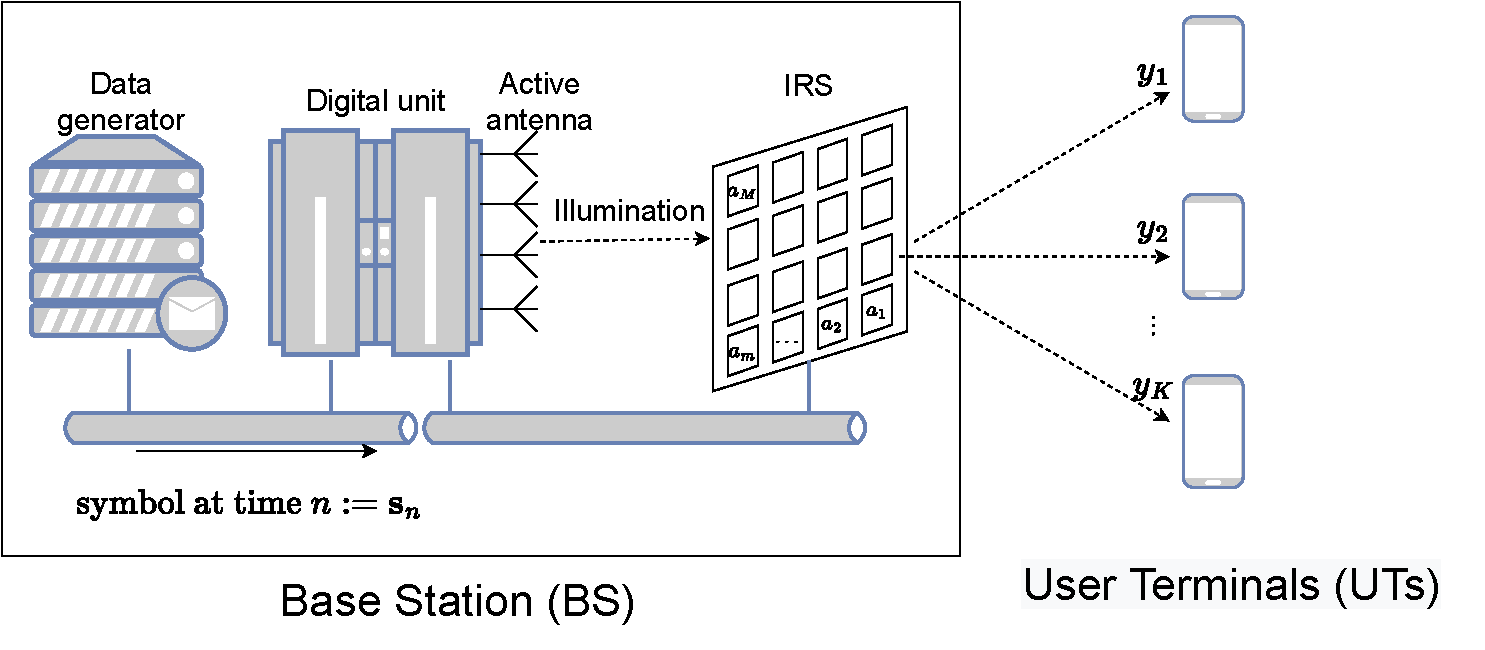
\includegraphics[width=6in]{sysmodel_illustration.pdf} 
	\caption{Illustration of the system model} \label{fig:sysmodel_illustration}
\end{figure}

\subsection{Block-Level Analog Beamforming}
While the digital unit can be updated at the symbol-level, the analog unit is updated once per a block of symbol intervals. From the implementational viewpoint, this means that the signals on the illuminators are updated once every symbol interval, but the phase-shifts at \ac{irs} are updated only once at the beginning of a transmission block. Fig. \ref{fig:abssys} depicts this block-level transmission strategy. In this figure, the table entries with the same color correspond to the message symbols of the same block. %For example, the RF chain output vectors from time interval $L+1$ to $2L$ are computed based on the buffered message vectors generated from time interval $1$ to $L$. Besides, if we 
Assuming that the information symbol rate to be $R$, the \ac{rf}-chains are updated at rate $R$ while the \ac{irs} is tuned at the rate $R/L$.
\begin{figure}[t]\flushleft
	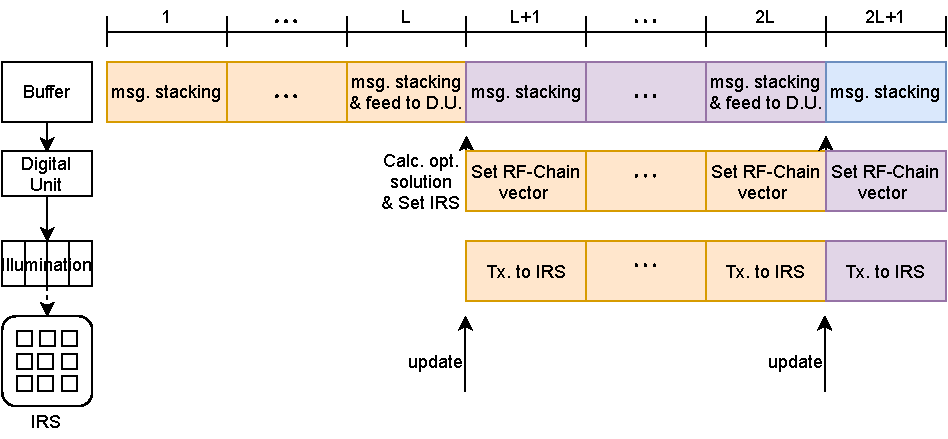
\includegraphics[width=6in]{modeltime.pdf} 
	\caption{Transmitter Time Table} \label{fig:abssys}
\end{figure}

Let $\mathbf S$ denote the collection of information symbols being transmitted in a particular block. This can be written as 
\begin{equation}
	\mathbf S=\left[ \mathbf s_1, \mathbf s_2, \cdots,  \mathbf s_L\right] ,
\end{equation}
with $L$ being the block length. %and $\mathbf{s}_\ell$ denotes the vector of encoded data sent in the $\ell$-th symbol interval of the block to the \acp{ut}. %
%with $\mathbf s_\ell=\left[ s_1, s_2, \cdots, s_K \right]^{\mathsf{T}} $ being the message symbol for  the $K$ \acp{ut} at the $\ell$-th time interval and $L$ denotes the block size of block-wise precoder. This can be achieved by attaching a buffer to the data generator. The transmitted signal first passes through the \ac{rf} chains, let denote the output of \ac{rf}-chains with $\mathbf X\in \mathbb C^{N\times L_X}$, and then delivers to the \ac{irs} which is placed sufficiently close to the active antennas. With this assumption, the illumination channel from the RF chains to the IRS can be considered fixed during the entire transmission. 
We assume that the block length $L$ is smaller than the coherence time interval of the channel, as it is the case in practice. This means that the channel coefficients can be considered to remain unchanged during signal transmission in a single block. As a result, the matrix of signals received in this block at the \acp{ut}, i.e., 
\begin{align}
	\mathbf Y=\left[ \mathbf y_1, \mathbf y_2 \cdots  \mathbf y_L\right],
\end{align}
is given by
 \begin{equation}
	\mathbf Y=\mathbf{H}^\trp \mathbf{A} \mathbf{T} \mathbf{X}+\mathbf{W}, 
\end{equation}
%where $\mathbf H\in \mathbb C^{K\times M}$ denotes the channel matrix from base station to the \acp{ut}, 
%$\mathbf A=\mathrm{diag}\{e^{j\beta_1}, \dots, e^{j\beta_M}\}$ with $0\leq \beta_m\leq 1$ modeling the phase-shifts which applies by the passive elements of the \ac{irs}, $\mathbf T \in \mathbb C^{M\times N}$ represents the illumination channel from the \ac{rf}-chains to the \ac{irs}, and 
where $\mathbf{X}=\dbc{\mathbf x_1,  \dots, \mathbf x_L }$ denotes the digitally-precoded transmit signals in the block, and $\mathbf{W}=\dbc{\mathbf w_1,  \dots, \mathbf w_L }$. Here, we drop the time index $\ell$ for the analog phase-shifters and the channel coefficients as they remain unchanged during the block transmission.
%$\mathbf W=[\mathbf W_1, \mathbf W_2, \cdots, \mathbf W_N]$ denotes the additive white Gaussian noise matrix whose columns follow \ac{iid} Gaussian distribution with zero mean and variance $\sigma_n^2$, i.e., $\sigma_n^2=\mathcal{CN}\left(\mathbf 0, \sigma_n^2 \mathbf I_K \right) $.
%To keep the \acp{ut} simple and  reduce the hardware complexity and computational power, a disjoint decoder is considered for \acp{ut}. 
%Consequently, the decoded signal $\tilde{\mathbf Y}\in \mathbb C^{K\times L}$ is given by

%\cmt{I noticed that we use $n$ for both RF-chain index and time index above. This is confusing. Please change all of the time indices above to $\ell$.}

\subsection{Linear Reception}
At the receiver side, we assume a simple post-processing strategy: as \ac{ut} $k$ receives the symbol $y_{k,\ell}$ in interval $\ell$ of the block, it takes its scaled version $\tilde{y}_{k,\ell} = F_k y_{k,\ell}$ as the soft estimate of the transmitted symbol $s_{k,\ell}$. The receiver gains of the \acp{ut} are updated based on channel statistics and hence remain unchanged within a coherence time interval. As the result, we can represent the matrix of soft estimates collected by the \acp{ut} within the transmission block as
\begin{equation}
	\tilde{\mathbf Y}=\mathbf F \mathbf Y, %=\mathbf S.
\end{equation}
where $\mathbf{F} = \Diag{ F_1, \ldots, F_K }$. In our transmission scheme, we assume that the elements of the matrix $\mathbf F$ compensate for the path loss.%denote the disjoint decoder and it is assumed that it is a diagonal matrix. Moreover, to keep the decoded signal as close as possible to the intended message, it is assumed that $\mathbf Y$ and $\mathbf S$ have the same dimension, i.e., $L_X=L$.


%\subsection{Channel Estimation}
%\cmt{This part moves up where I asked to present the CSI acquisition procedure. Please merge it properly there.}
%\par In practical scenarios, \acp{bs} generally access the imperfect \ac{csi} due to the channel estimation and quantization errors. In this paper, the channel uncertainties are assume to follow the expectation-based model given by \cite{gershman2010convex}
%\begin{equation}
%	\mathbf H=\hat{\mathbf H}+\mathbf E,
%\end{equation}
%where $\hat{\mathbf H}\in\mathbb C^{K\times M}$ is the estimated channel matrix and $\mathbf E\in\mathbb C^{K\times M}$ denotes the channel uncertainty. In statistical model, it is assumed that the entries of the error matrix $e_{k, m}=\left[ \mathbf E\right]_{k, m}$ are Gaussian distributed, i.e.,  $e_{k,m}\sim \mathrm{CN}(0, \sigma_{\mathrm{e}, k}^2)$. Moreover, we assume that $e_{k,m}$ are independently and user-wise/row-wise-identically distributed with $\mathbb E\{e_{k,m}\}=0$ and $\mathbb E\{e_{k_1,m_1}^*e_{k_2,m_2}\}=\sigma_{\mathrm{e}, k_1}^2\delta(k_1-k_2)\delta(m_1-m_2)$.


%%%%%%%%%%%%%%
%\textcolor{blue}{The next section is channel modeling, but I wasn't sure if we need to explain it here. Because the channel model is mainly used in the numerical result part. So, we can shift it to that section.}
%%%%%%%%%%%%%%%%

% the vector of the received signals in this network in the $i$-th symbol time instance drawn from a block is given by
%\begin{equation}
%\mathbf y_i=\mathbf H\mathbf a_i+\mathbf W_i,
%\label{eq:basic}
%\end{equation}
%where $\mathbf H\in \mathbb C^{K\times M}$ is the wireless channel matrix from base station to all the \acp{ut} if the \ac{csi} is known. The received vector is written as 
%\begin{equation}
%\mathbf y_i=\begin{bmatrix}y_1 & \dots & y_K\end{bmatrix}^{\mathsf{T}},
%\end{equation}
%where $y_k$ denotes the signal at the $k$-th \ac{ut}. Vector $\mathbf a_i\in \mathbb C^{M\times 1}$ represents the signals transmitted by the \ac{bs} and $\mathbf W_i$ is a $K$ by one noise vector whose entries are i.i.d. drawn from Gaussian distribution with zero mean and variance $\sigma_n^2$. 
%
%\begin{figure}[htbp]\flushleft
%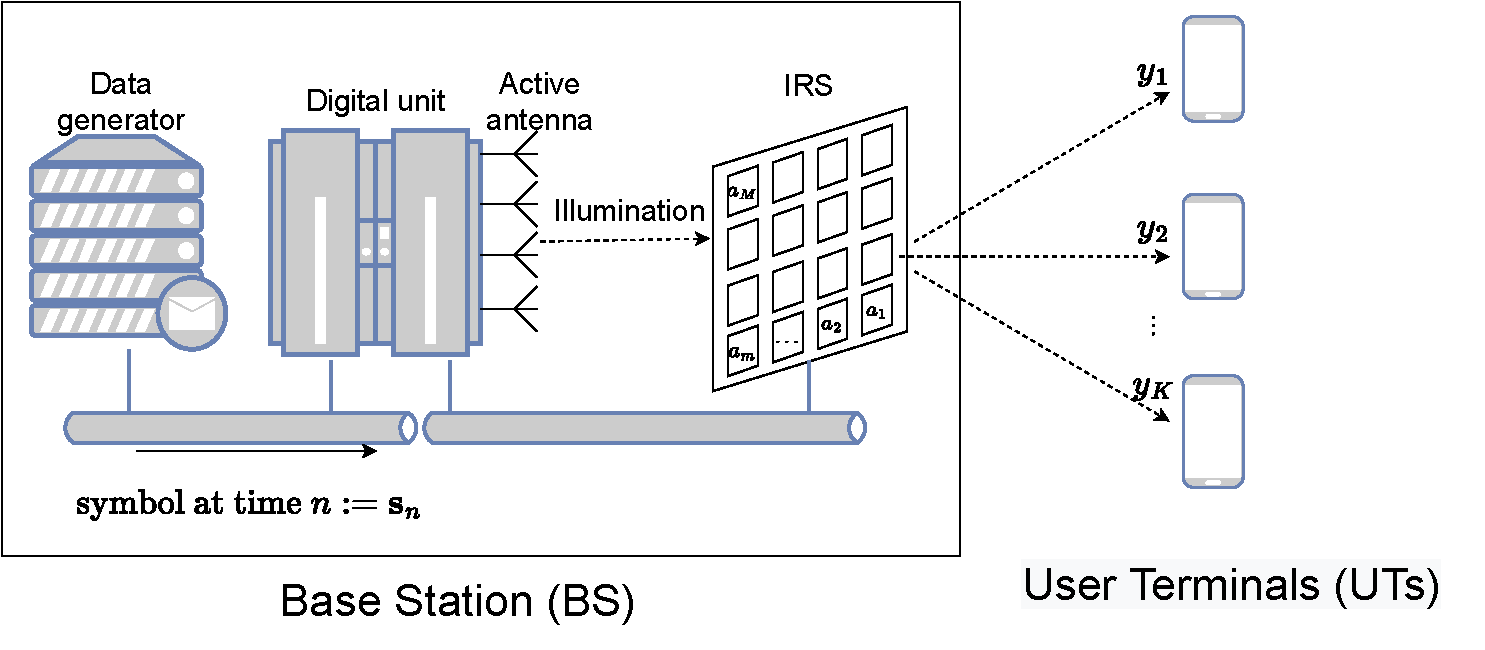
\includegraphics[width=6in]{sysmodel_illustration.pdf} 
%\caption{System Model} \label{fig:sysgen}
%\end{figure}
%The \ac{bs} employs an \ac{irs}-aided HAD transmitter whose architecture is demonstrated in Fig. (\ref{fig:sysgen}).
%
%Define $s_k$ as the message symbol intended for the $k$-th \ac{ut}, and the message vector for all the $K$ \acp{ut} at the $i$-th time interval can be denoted as 
%\begin{equation}
%\mathbf s_i=\begin{bmatrix}s_1 & \dots &s_K\end{bmatrix}^{\mathsf{T}}.
%\end{equation}
%In this paper, block-wise precoding  with block size $L$ is used. This can be achieved by attaching a buffer to the data generator. The message for one entire block is represented as 
%\begin{equation}
%\mathbf S=\begin{bmatrix}\mathbf s_1 & \dots & \mathbf s_L\end{bmatrix}. 
%\end{equation}
%Similarly, the transmitted signal and the received signal in one block can be modeled respectively as follow,
%\begin{equation}
%\begin{split}
%\mathbf A&=\begin{bmatrix}\mathbf a_1 & \dots & \mathbf a_L\end{bmatrix}\\
%\mathbf Y&=\begin{bmatrix}\mathbf y_1 & \dots & \mathbf y_L\end{bmatrix}.
%\end{split}
%\end{equation}
%Therefore, the block-wise system model is described by
%\begin{equation}
%\mathbf Y=\mathbf H\mathbf A+\mathbf W,
%\end{equation}
%where $\mathbf W$ is a $K\times N$ random matrix standing for the noise. Next, we are going to discuss the transmitter output matrix $\mathbf A$ and channel matrix $\mathbf H$ as well as the decoder in more detail.
%\subsection{Transmitter Architecture}
%\cmt{This part moves up where I asked to present the CSI acquisition procedure. Please merge it properly there.}
%An illustration for the internal structure of the \ac{bs} with $N$ RF chains and $M$ passive \ac{irs} elements is shown as Fig. (\ref{fig:detailsys}).
%\begin{figure}[htbp]\flushleft
%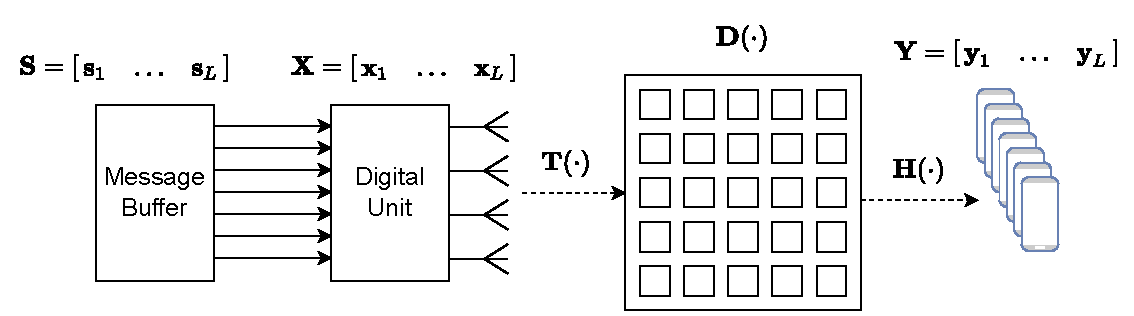
\includegraphics[width=6in]{siggram.pdf} 
%\caption{Signal diagram of the Base Station} \label{fig:detailsys}
%\end{figure}
%If the matrix $\mathbf S$ contains the intended messages for the \acp{ut} during one transmission time block, we can define a matrix $\mathbf X\in \mathbb C^{N\times L_X}$ to be the RF chain output signals corresponding to that message matrix. Additionally, the phase-shifts of the \ac{irs} for this message block are contained by $\mathbf A=\mathrm{diag}\{e^{j\beta_1}, \dots, e^{j\beta_M}\}$. The \ac{irs} is placed in the close proximity of the active antennas, and the illumination channel from the RF chains to the IRS can be considered as fixed during the entire transmission. This fixed channel is denoted as a constant matrix $\mathbf T \in \mathbb C^{M\times N}$.
%
%Since the \acp{ut} are disjoint and don't possess the same computational power as the base station,  they can only employ a simple disjoint decoder. The disjoint decoder can be modeled as a diagonal matrix $\mathbf F_{\mathrm{D}}$, i.e. 
%\begin{equation}
%\tilde{\mathbf Y}=\mathbf F_{\mathrm{D}}\mathbf Y=\mathbf S.
%\end{equation}
%
%By considering the internal structure of the transmitter, the matrix for the received signals $\mathbf Y$ can also be represented as 
% \begin{equation}
% \mathbf Y=\mathbf {HATX}+\mathbf{N}.
% \label{eq:sysmain}
% \end{equation}
%
%To make the decoded signal as close as possible to the intended message, $\mathbf Y$ and $\mathbf S$ must have the same dimension. Therefore, the matrix $\mathbf X$ must have as many columns as matrix $\mathbf S$. Thus, we have $L_X=L$ and $\mathbf X\in \mathbb C^{N\times L}$.
% 
%In block-wise precoding, we apply the same phase-shifts matrix $\mathbf A$ to all the digital-domain vectors contained in the same time block. In this way, the active antennas are updated once every symbol time interval, but the \ac{irs} only updates once every time block.
% 
%This transmission procedure can be illustrated in Fig. (\ref{fig:abssys}).
%\begin{figure}[htbp]\flushleft
%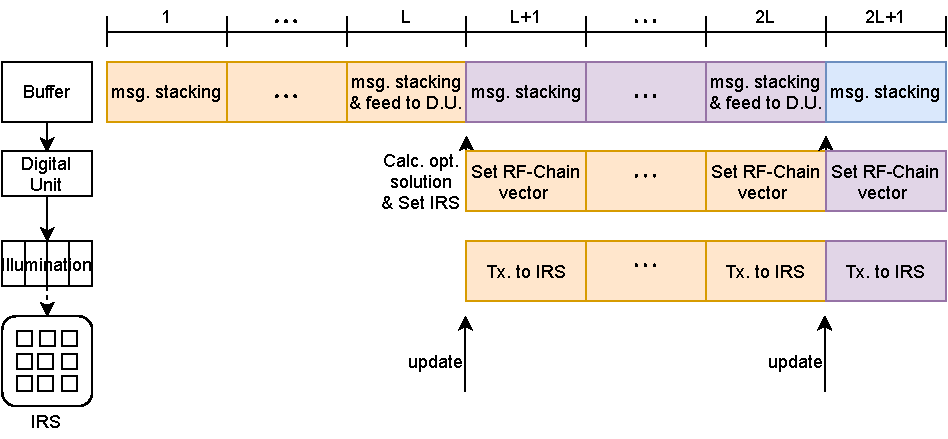
\includegraphics[width=6in]{modeltime.pdf} 
%\caption{Transmitter Time Table} \label{fig:abssys}
%\end{figure}
%In Fig. (\ref{fig:abssys}), the table entries with the same color indicate that they all correspond to the message symbols of the same block. For example, the RF chain output vectors from time interval $L+1$ to $2L$ are computed based on the buffered message vectors generated from time interval $1$ to $L$. 
%
%If the message vectors are generated at the rate $R$ then the symbol time interval is $T_{\mathrm{s}}=1/R$. It can be observed that the RF chain output also has the same update rate but with a delay of $LT_{\mathrm{s}}$ relative to the corresponding messages. Compared to symbol-wise transmission, the \ac{irs} is reconfigured once per time block, so its update rate is only $R/L$.





\subsection{Performance Metrics and Design Objectives}
The main objective of this work is to design the digital and analog units oft the transmitter, i.e., $\Pi_\ell\brc{\cdot}$ and $\mathbf{A}$, such that the system throughput is optimized. To this end, we need to introduce some performance measures for the evaluation. One commonly used designing criteria is achievable rate per user, which is bounded by \cite{sedaghat2017novel}:
\begin{equation}
\bar R\geq \frac{LT_{\mathrm{s}}}{\tau+LT_{\mathrm{s}}}\log\left(1+\frac{\sigma_s^2}{P_{\mathrm{Noise}}+P_{\mathrm{Interference}}}\right),
\end{equation}
where $T_{\mathrm{s}}$ is symbol time, $\tau$ is the duration of guard interval and $P_{\mathrm{Interference}}$ is the average interference power after the decoding/compensation process. The power term $P_{\mathrm{Noise}}$ is the equivalent noise after reception. The variance $\sigma_s^2$ is the power of the information data. 

For a system with fixed block length, $\Pi_\ell\brc{\cdot}$ and $\mathbf{A}$ only have influence on $P_{\mathrm{Interference}}$. Thus, the \ac{rss} can be adopted here to assess the distortion between the decoded signals and the intended messages. It is defined as
\begin{equation}
\mathrm d(\mathbf S, \tilde{\mathbf Y})=||\tilde{\mathbf Y}-\mathbf S||_{\mathrm{F}}^2=\mathrm{tr}\{(\tilde{\mathbf Y}-\mathbf S)^{\mathsf H}(\tilde{\mathbf Y}-\mathbf S)\}.
\label{eq:distancegeneral}
\end{equation}
 It is desired to make $\tilde{\mathbf Y}$ similar to the coded message symbols $\mathbf S$. In the following two sections, we will try to develop an algorithm to configure the digital precoder $\Pi_\ell$ and analog precoder $\mathbf A$ jointly for arbitrary block length $L$ to optimize the throughput.


\section{Precoding via Least-Squares Method}
In Eq.(\ref{eq:distancegeneral}), $\mathbf F$ is used to compensate for the path loss which is defined in matrix form as
\begin{equation}
\mathbf P_{\mathrm L}^{1/2}=
\begin{bmatrix}
\sqrt{\bar h_1} & & \\
&\ddots & \\
& &\sqrt{\bar h_K}
\end{bmatrix},
\end{equation}
where $\bar h_{1\dots K}$ denotes the path loss between the \ac{bs} and \acp{ut}.
The decoder/compensator can then be designed as 
\begin{equation}
\mathbf F=\mathbf P_{\mathrm L}^{-1/2}.
\end{equation}
Thus, the compensated received signal is
%\begin{equation}
%\tilde{\mathbf Y}=\mathbf P_{\mathrm L}^{-1/2}\mathbf Y.
%\end{equation}

%\subsection{Statistics of the Performance Measure}
%Most of times, the channel estimation is imperfect. The relation between real channel and estimated channel can be described by the following equation,
%\begin{equation}
%\mathbf H=\hat{\mathbf H}+\mathbf E,
%\end{equation}
%where $\mathbf H \in \mathbb C^{K\times M}$ stands for the real channel, $\hat{\mathbf H}\in\mathbb C^{K\times M}$ is the estimated channel and their difference is modeled as a $K$ by $M$ complex random matrix $\mathbf E$. We assume here that each entry of the error matrix are independently and user-wise/row-wise-identically distributed following the two statistics in Eq. (\ref{eq:errorstatistics}).
%\begin{equation}
%\begin{split}
%&\mathcal E\{e_{k,m}\}=0;\\
%&\mathcal E\{e_{k_1,m_1}^*e_{k_2,m_2}\}=\sigma_{\mathrm{e}, k_1}^2\delta(k_1-k_2)\delta(m_1-m_2).
%\label{eq:errorstatistics}
%\end{split}
%\end{equation}
%The random variable $e_{k,m}\sim \mathrm{CN}(0, \sigma_{\mathrm{e}, k}^2)$ denotes the entry at the $k$-th row and the $m$-th column of matrix $\mathbf E$. 
%The $\delta(\cdot)$ is the discrete Dirac function which is evaluated to zero when it has non-zero argument and evaluate to one when its argument is zero.
%
%Taking the estimation error into consideration, the received signals and the decoded/compensated signals can then be written as 
\begin{equation}
\begin{split}
%\mathbf Y=&(\hat{\mathbf H}^{\mathsf T}+\mathbf{E}^{\mathsf T})\mathbf{ATX}+\mathbf W\\
\tilde{\mathbf Y}=\mathbf P_{\mathrm L}^{-1/2}[( \hat{\mathbf H}^{\mathsf T}+\mathbf{E}^{\mathsf T})\mathbf{ATX}+\mathbf W].
 \label{eq:channelmodelwithestimationerror}
\end{split}
\end{equation}

To keep the further discussions brief, define the normalized matrices $\tilde{\mathbf H}$, $\tilde{\hat{\mathbf H}}$, $\tilde{\mathbf E}$ and $\tilde{\mathbf W}$ as  Eq. (\ref{eq:compensatednotations}).
\begin{equation}
\begin{split}
\tilde{\mathbf H}=		&\mathbf P_{\mathrm L}^{-1/2}{\mathbf H}\\
\tilde{\hat{\mathbf H}}^{\mathsf T}=	&\mathbf P_{\mathrm L}^{-1/2}{\hat{\mathbf H}}^{\mathsf T}\\
\tilde{\mathbf E}^{\mathsf T}=		&\mathbf P_{\mathrm L}^{-1/2}{\mathbf E}^{\mathsf T}\\
\tilde{\mathbf W}=		&\mathbf P_{\mathrm L}^{-1/2}{\mathbf W}
\end{split}
\label{eq:compensatednotations}
\end{equation}


Because of the existence of random terms, statistics of Eq. (\ref{eq:distancegeneral}) are used for the designing. Assume that the noise entries are independent with the estimation errors, we then have
\begin{equation}
\begin{split}
&\mathcal E_{\mathbf E}\left\{\mathcal E_{{\mathbf W}}\{\mathrm d(\mathbf S, \tilde{\mathbf Y})\}\right\}\\
=&\left|\left|\tilde{\hat{\mathbf{H}}}^{\mathsf T}\mathbf{ATX}-\mathbf{S}\right|\right|_{\mathrm{F}}^2+\mathrm{tr}\{\mathbf X^{\mathsf H}\mathbf T^{\mathsf H}\mathbf A^{\mathsf H}
\pmb{\Sigma_{\tilde{\mathbf E}}}\mathbf{ATX}\}+L\mathrm{tr}\{\mathbf P_{\mathrm L}^{-1}\}\sigma_{\mathrm n}^2,
\end{split}
\label{eq:basedis}
\end{equation}
where
\begin{equation}
\pmb{\Sigma_{\tilde{\mathbf E}}}=
%\begin{bmatrix}
%\sum_{k=1}^K \sigma_{\mathrm e, k}^2/\bar{h}_k &&\\
%&\ddots &\\
%&&\sum_{k=1}^K \sigma_{\mathrm e, k}^2/\bar{h}_k
%\end{bmatrix}=\
sum_{k=1}^K \sigma_{\mathrm e, k}^2/\bar{h}_k\cdot \mathbf{I}_M.
\end{equation}
The formula given in Eq. (\ref{eq:basedis}) is the expected distance between $\mathbf S$ and $\tilde{\mathbf Y}$, i.e. $\mathcal E_{\mathbf W, \mathbf E}\{\mathrm d(\mathbf S, \tilde{\mathbf Y})\}$. From now on, instead of developing an algorithm that minimize Eq. (\ref{eq:distancegeneral}) directly, we try to develop an algorithm that minimize Eq. (\ref{eq:basedis}) by optimizing $\mathbf A$ and $\mathbf X$.

\subsection{Problem Formulation as a GLSE Precoder}
Following \cite{glse}, if we utilize the peak and total power limitation, the minimization of the expected distance between the intended message and the received symbols leads us to the design of a GLSE precoder. The optimization problem is given by
\begin{equation}
\begin{aligned}
& \underset{\mathbf A, \mathbf X}{\text{minimize}}
& &\left|\left|\tilde{\hat{\mathbf H}}^{\mathsf T}\mathbf{ATX}-\mathbf{S}\right|\right|_{\mathrm{F}}^2+\mathrm{tr}\{\mathbf X^{\mathsf H}\mathbf T^{\mathsf H}\mathbf A^{\mathsf H}
\pmb{\Sigma_{\tilde{\mathbf E}}}\mathbf{ATX}\}+\lambda\mathrm{tr}\{\mathbf X\mathbf X^{\mathsf H}\}\\
& \text{subject to}
& &\max_{i,j} |x_{i,j}|^2<P_{\mathrm{peak}},
%& & &\mathrm{tr}\{\mathbf{XX}^{\mathsf H}\}\leq P_{\mathrm{total}}.
\label{opt:raw}
\end{aligned}
\end{equation}
where $P_{\mathrm{peak}}\geq 0$ is the peak power constraint. Another variable $\lambda\geq 0$ represents the regularizer that balences the trade-off between the expected distance and total transmission power. With larger $\lambda$, the system will have to put more emphasis on constraining the total transmission power. On the contrary, with smaller $\lambda$, the system will pay more attention to minimize the expected distortion between received signals and intended signals. 

The peak power constraint can be adjusted along with the regularizer to control the \ac{papr}.
To keep the discussion brief, $\mathrm{obj}(\cdot)$ is used to denote the objective function in Eq. (\ref{opt:raw}). It is defined as
\begin{equation}
\begin{split}
\mathrm{obj}(\mathbf A, \mathbf X, \mathbf S)&=\left|\left|\tilde{\hat{\mathbf H}}^{\mathsf T}\mathbf{ATX}-\mathbf{S}\right|\right|_{\mathrm{F}}^2+\mathrm{tr}\{\mathbf X^{\mathsf H}\mathbf T^{\mathsf H}\mathbf A^{\mathsf H}
\pmb{\Sigma_{\tilde{\mathbf E}}}\mathbf{ATX}\}+\lambda\mathrm{tr}\{\mathbf X\mathbf X^{\mathsf H}\}
\label{eq:objfunc}
\end{split}
\end{equation}
The term $L\mathrm{tr}\{\mathbf P_{\mathrm L}^{-1}\}\sigma_{\mathrm n}^2$ is removed from the objective function, because it is a constant term that depends neither on $\mathbf A$ nor on $\mathbf X$.

\section{GLSE Precoding via Alternating Optimization}
The joint optimization of the problem stated in (\ref{opt:raw}) is non-trivial since it is generally non-convex. Alternating optimization method is adopted to obtain a suboptimal solution iteratively. In each iteration, the optimal RF chain outputs are first calculated while treating the IRS configurations as a fixed matrix, and then the system looks for a suitable (may not be optimal) phase-shifts configuration while treating $\mathbf X$ as a fixed matrix. The pseudo-code in Algorithm (\ref{algo:jointalgorithm}) depicts the general procedure. 
\begin{algorithm}
\caption{General Procedure for finding ($\mathbf{A}$, $\mathbf{X}$)}
\begin{algorithmic}[1]
\State $ (\mathbf{A}, \mathbf{X}) \gets \mathrm{initial\ values} $
\While {terminate condition not met}
\State $\mathbf{X}\gets \mathop{\arg\min}_{\mathbf{X}}\ \mathrm{obj}(\mathbf A, \mathbf X, \mathbf S)\ \mathrm{s.t.}\ \max_{i,j} |x_{i,j}|^2<P_{\mathrm{peak}} $ 
\State $\mathbf{A}\gets \mathop{\arg\min}_{\mathbf{A}}\ \mathrm{obj}(\mathbf A, \mathbf X, \mathbf S)$
\EndWhile
\end{algorithmic}
\label{algo:jointalgorithm}
\end{algorithm}

A termination condition for the loop should be chosen accordingly. For example, let the loop be executed until two consequent loops have their cost function difference smaller than a certain threshold or terminates when certain iteration time is reached. The step 3 in the algorithm (optimize with respect to $\mathbf X$) is quadratic programming, which is categorized as convex optimization problem. Therefore, an optimal $\mathbf X$ can always be obtained if $\mathbf A$ is given. 

The domain of $\mathbf A$ is not a convex set. This implies that the step 4 in the algorithm is a non-convex problem. Thus, the optimal value in step 4 can generally not be found. This leads to a problem that Algorithm (\ref{algo:jointalgorithm}) may not converge, because in step 4, the system may find a suboptimal minimal for $\mathbf A$ that may lead to a larger cost than the previous iteration. 

\subsection{Optimization of the Digital Unit}
When $\mathbf A$ is treated as a fixed matrix, the problem given by
\begin{equation}
\begin{aligned}
& \underset{\mathbf X}{\text{minimize}}
& &\left|\left|\tilde{\hat{\mathbf H}}^{\mathsf T}\mathbf{ATX}-\mathbf{S}\right|\right|_{\mathrm{F}}^2+\mathrm{tr}\{\mathbf X^{\mathsf H}\mathbf T^{\mathsf H}\mathbf A^{\mathsf H}
\pmb{\Sigma_{\tilde{\mathbf E}}}\mathbf{ATX}\}+\lambda\mathrm{tr}\{\mathbf X\mathbf X^{\mathsf H}\}\\
& \text{subject to}
& &\max_{i,j} |x_{i,j}|^2<P_{\mathrm{peak}}
%& & &\mathrm{tr}\{\mathbf{XX}^{\mathsf H}\}\leq P_{\mathrm{total}}.
\label{opt:rfcopt}
\end{aligned}
\end{equation}
belongs to the class of convex problem. Moreover, it is worth noticing that the columns (time intervals) of matrix $\mathbf X$ can be decoupled according to Eq. (\ref{eq:decouple}).
\begin{equation}
\begin{split}
\mathrm{tr}\{(\tilde{\hat{\mathbf H}}^{\mathsf T}\mathbf{ATX}-\mathbf{S})^{\mathsf H}(\tilde{\hat{\mathbf H}}^{\mathsf T}\mathbf{ATX}-\mathbf{S})\}+\mathrm{tr}\{\mathbf X^{\mathsf H}\mathbf T^{\mathsf H}\mathbf A^{\mathsf H}
\pmb{\Sigma_{\tilde{\mathbf E}}}\mathbf{ATX}\}+\lambda \mathrm{tr}\{\mathbf{X}^{\mathsf H}\mathbf{X}\}\\
=\sum_{i=1}^L(\tilde{\hat{\mathbf H}}^{\mathsf T}\mathbf{AT}\boldsymbol{x_i}-\boldsymbol{s_i})^{\mathsf H}(\tilde{\hat{\mathbf H}}^{\mathsf T}\mathbf{AT}\boldsymbol{x_i}-\boldsymbol{s_i})+
\mathbf x_i^{\mathsf H}\mathbf T^{\mathsf H}\mathbf A^{\mathsf H}
\pmb{\Sigma_{\tilde{\mathbf E}}}\mathbf{ATx}_i
+\lambda \boldsymbol{x_i}^{\mathsf H}\boldsymbol{x_i}.
\label{eq:decouple}
\end{split}
\end{equation}

Therefore, this optimization problem can either be treated as one matrix convex optimization or $L$ independent vector convex optimization problems. This implies that the block length has no influence over the RF chain outputs if $\mathbf A$ is fixed. 
%graph here
%\

\subsection{Optimization of the IRS Configuration}
When treating $\mathbf X$ as a fixed matrix, the optimization problem is then formulated as
\begin{equation}
\begin{aligned}
& \underset{\mathbf A}{\text{minimize}}
& &\left|\left|\tilde{\hat{\mathbf H}}^{\mathsf T}\mathbf{ATX}-\mathbf{S}\right|\right|_{\mathrm{F}}^2+\mathrm{tr}\{\mathbf X^{\mathsf H}\mathbf T^{\mathsf H}\mathbf A^{\mathsf H}
\pmb{\Sigma_{\tilde{\mathbf E}}}\mathbf{ATX}\}.\\
\label{opt:irsopt}
\end{aligned}
\end{equation}
It is generally non-convex problem, since the domain of $\mathbf A$ is not a convex set. Two methods are used here to obtain a suboptimal point, which are gradient descent and \ac{mm} algorithm \cite{sankuru2020designing}. For further discussions, we denote the objective function in Eq. (\ref{opt:irsopt}) by
\begin{equation}
\begin{split}
\mathrm{obj}_{\mathbf A}(\mathbf A)=\left|\left|\tilde{\hat{\mathbf H}}^{\mathsf T}\mathbf{ATX}-\mathbf{S}\right|\right|_{\mathrm{F}}^2+\mathrm{tr}\{\mathbf X^{\mathsf H}\mathbf T^{\mathsf H}\mathbf A^{\mathsf H}
\pmb{\Sigma_{\tilde{\mathbf E}}}\mathbf{ATX}\}.
\label{eq:objectivefunctionofirs}
\end{split}
\end{equation}

\subsubsection{Gradient descent method}
Gradient descend is a general method to find the local optimal of the functions that maps one or multiple parameters to $\mathbb R$. The local minimal can be obtained by following the opposite gradient of the function iteratively from a random initial point. This can be understood graphically as following the steepest slope on a surface until reaching the trough.

In order to simplify the domain, define the phase vector
\begin{equation}
\boldsymbol \beta=\arg \cdot \mathrm{diag_{vector}}(\mathbf A).
\end{equation}
To keep the notation simple, we declare auxiliary matrices as follow
\begin{equation}
\begin{split}
\mathbf U&= \mathbf{ATX};\\
\mathbf V&=\mathbf S^{\mathsf H}\tilde{\hat{\mathbf H}}^{\mathsf T}\\
\mathbf Q&=\tilde{\hat{\mathbf H}}^*\tilde{\hat{\mathbf H}}^{\mathsf T}+
\pmb{\Sigma_{\tilde{\mathbf E}}}.
\end{split}
\label{eq:irsgdsimplifiedsymbols}
\end{equation}
Under this convention, the objective function can be expanded as 
\begin{equation}
\mathrm{obj_{\mathbf A}}(\mathbf A)=\mathrm{tr}\{\mathbf U^{\mathsf H}\mathbf Q \mathbf U- (\mathbf U^{\mathsf H}\mathbf V^{\mathsf H}+\mathbf{VU})+\mathbf S^{\mathsf H}\mathbf S\}.
\label{eq:simplifiedirsobj}
\end{equation}
Since the differential operation is linear, we first calculate the the derivative of the additive terms in Eq. (\ref{eq:simplifiedirsobj}) as
\begin{equation}
\begin{split}
\frac{\partial \mathrm{tr}\{\mathbf U^{\mathsf H}\mathbf Q \mathbf U\}}{\partial\boldsymbol\beta} &= -2\mathrm{diag_{vector}}(\Im(\mathbf{UU^{\mathsf H}Q}))\\
\frac{\partial{\mathrm{tr}\{\mathbf U^{\mathsf H}\mathbf V^{\mathsf H}+\mathbf{VU}\}}}{\partial{\boldsymbol{\beta}}} &= -2\mathrm{diag_{vector}}(\Im(\mathbf{UV})).
\end{split}
\label{eq:partialderivertivesplit}
\end{equation}

From Eq. (\ref{eq:simplifiedirsobj}) and Eq. (\ref{eq:partialderivertivesplit}), the partial derivative of the objective function can be derived as

\begin{equation}
\frac{\partial \mathrm{obj_{\mathbf A}}(\mathbf A)}{\partial\boldsymbol\beta} = -2\mathrm{diag_{vector}}(\Im(\mathbf{UU^{\mathsf H}Q}-\mathbf{UV})).
\label{eq:partialderivertivetotal}
\end{equation}

The auxiliary vector can be transformed back to the phase-shift matrix by Eq. (\ref{eq:irsphaseinversetransformation}).

\begin{equation}
\mathbf A=\mathrm{diag_{matrix}}\left(\mathrm{exp}({j\boldsymbol \beta})\right)
\label{eq:irsphaseinversetransformation}
\end{equation}

Combining with the designing of the digital unit, the pseudo-code of the precoding algorithm with gradient descent is shown as Algorithm (\ref{algo:gradientdescentfull}).
\begin{algorithm}
\caption{Precoding ($\mathbf{A}$, $\mathbf{X}$) with gradient descent}
\begin{algorithmic}[1]
\State $ (\mathbf{A}, \mathbf{X}) \gets \mathrm{initial\ values} $
\While {terminate condition not met}
\State $\mathbf{X}\gets\mathrm{convex_{opt}}\{\mathrm{obj}(\mathbf A, \mathbf X, \mathbf S)\ \mathrm{s.t.}\ \max_{i,j} |x_{i,j}|^2<P_{\mathrm{peak}}\}$
\While {terminate condition not met}
	\State $\boldsymbol \beta \gets \arg \cdot \mathrm{diag_{vector}}(\mathbf A)$
	\State $\boldsymbol \beta_\mathrm{grad}\gets -2\mathrm{diag_{vector}}(\Im(\mathbf{UU^{\mathsf H}Q}-\mathbf{UV}))$
	\State $\alpha \gets \mathrm{getStepSize}$
	\State $\boldsymbol \beta'=\boldsymbol \beta-\alpha \boldsymbol \beta_\mathrm{grad}$
	\State $\mathbf A\gets \mathrm{diag_{matrix}}\left(\mathrm{exp}({j\boldsymbol \beta'})\right)$
\EndWhile
%\State $\mathbf{A}=\mathrm{convex_{opt}}\mathop{\arg\min}_{\mathbf{A}}\ \mathrm{tr}\{(\mathbf{HATX}-\mathbf{S})(\mathbf{HATX}-\mathbf{S})^{\mathsf H}\}$
\EndWhile
\end{algorithmic}
\label{algo:gradientdescentfull}
\end{algorithm}

In order to avoid the situation where the algorithm diverges, one can design the step size $\alpha$ in the following steps. At the beginning of each gradient descent loop (step 4 - 10 in Algorithm (\ref{algo:gradientdescentfull})), $\alpha$ is initialized to a relative large value. During each loop, the processor keeps the old value of $\mathbf A$ in the memory. If the value of the objective function does not decrease with the new $\mathbf A$, the processor will then load the old value of $\mathbf A$ from the memory and redo that gradient descent loop once again with halved step size. 

The whole gradient descent loop terminates if the value of $\alpha$ is smaller than a certain threshold. In this way, $\mathbf A$ will always be assigned to a value that makes the objective function decrease. Moreover, if the termination threshold for $\alpha$ is small enough, $\mathbf A$ will always end up at the close proximity of a critical point after the termination of one entire gradient descent loop. 

It is worth noticing that, though we can make the algorithm converge to a suboptimal point, it does not mean that the systems starting with different initial pairs $(\mathbf A, \mathbf X)$ will converge to the same value.  





\subsubsection{Majorize-minimization (MM) algorithm}
\ac{mm} algorithm  \cite{sankuru2020designing} is another general optimization method that can be used to optimize the IRS configurations. Similar to gradient descent, this algorithm also includes iterative procedures itself.  However, when using MM algorithm we don't need to state the step size explicitly.

A special auxiliary function called surrogate function $\overline{\mathrm{obj}_{\mathbf A_0}}:\mathrm{domain}(\mathrm{obj}(\cdot))\rightarrow \mathbb R$ is used in MM algorithm. It a less complicated function that need to be constructed at any point $\mathbf A_0$ of the objective function. The surrogate function constructed at a point must touch the objective function at that point. Meanwhile, it should always be larger or equal to the objective function at every point within its domain.

 The procedure of optimizing $\mathbf A$ with MM algorithm can be iteratively described as follow. At the $i$-th MM iteration for optimizing the IRS, a surrogate function of a point $\mathbf A_i$ is constructed. We then find the optimal point $\mathbf A_{i+1}$ that minimize the surrogate function. After that, we proceed to the next MM iteration and optimize a new surrogate function tangent to point $\mathbf A_{i+1}$. We can choose the initial point of $\mathbf A$ arbitrarily as long as it lies in the feasible set.


In oder to simplify the problem, we wish to construct a linear surrogate function free of quadratic terms. When expanded, the objective function in Eq. (\ref{eq:simplifiedirsobj}) is comprised of a quadratic term, two first order terms and one constant term with respect to $\mathbf A$. 

By the definition of surrogate function, the objective function is always a surrogate function of itself. The additive property of the surrogate functions can also be proven by the definition. This property states that two surrogate functions are additive if they are both tangent to their objective functions at the same point. Based on these two properties, a linear surrogate function for the objective function Eq. (\ref{eq:simplifiedirsobj}) can be constructed as follow. 

We first construct a linear surrogate function for the quadratic term of Eq. (\ref{eq:simplifiedirsobj}). The first order terms and constant term will serve as surrogate functions of themselves. The sum of those surrogate functions are the surrogate function for the whole objective function described by Eq. (\ref{eq:simplifiedirsobj}). Since the constant term does not contribute to the optimization, we can safely discard it.

Next we will give out the equivalent surrogate function.

To find the surrogate function, we use the auxiliary variables defined in Eq. (\ref{eq:irsgdsimplifiedsymbols}).
Furthermore, define

By substituting the variables according to Eq. (\ref{eq:irsgdsimplifiedsymbols}), the quadratic term can be written as
\begin{equation}
\begin{split}
\mathbf X^{\mathsf H}\mathbf T^{\mathsf H} \mathbf A^{\mathsf H}\left(\tilde{\hat{\mathbf H}}^{\mathsf H}\tilde{\hat{\mathbf{H}}}+\pmb{\Sigma_{\tilde{\mathbf E}}}\right)\mathbf{ATX}=\mathbf U^{\mathsf H} \mathbf{QU}.
\end{split}
\end{equation}

To construct the surrogate function for the quadratic term at an arbitrary point $\mathbf A_0$, we define an auxiliary matrix $\mathbf P$, such that $\mathbf P-\mathbf Q$ is positive definite. For the tangential point $\mathbf A_0$, we also define $\mathbf U_0=  \mathbf A_0\mathbf{TX}$. The surrogate for the quadratic term can be obtained by the following inequality \cite{sankuru2020designing}.
\begin{equation}
\begin{split}
	&\mathrm{tr}\left\{\mathbf U^{\mathsf H}\mathbf Q \mathbf U\right\}\\
=	&\mathrm{tr}\left\{\mathbf U_0^{\mathsf H} \mathbf Q \mathbf U_0+(\mathbf U-\mathbf U_0)^{\mathsf H} \mathbf Q\mathbf U_0+\mathbf U_0^{\mathsf H} \mathbf Q(\mathbf U-\mathbf U_0)+(\mathbf U-\mathbf U_0)^{\mathsf H}\mathbf Q(\mathbf U-\mathbf U_0)\right\}\\
\leq&\mathrm{tr}\left\{\mathbf U_0^{\mathsf H} \mathbf Q \mathbf U_0+(\mathbf U-\mathbf U_0)^{\mathsf H} \mathbf Q\mathbf U_0+\mathbf U_0^{\mathsf H} \mathbf Q(\mathbf U-\mathbf U_0)+(\mathbf U-\mathbf U_0)^{\mathsf H}\mathbf P(\mathbf U-\mathbf U_0)\right\}\\
=	&\mathrm{tr}\left\{\mathbf U^{\mathsf H}\mathbf P\mathbf U+\mathbf U^{\mathsf H}(\mathbf Q-\mathbf P)\mathbf U_0+ \mathbf U_0^{\mathsf H}(\mathbf Q-\mathbf P)\mathbf Y+\mathbf U_0^{\mathsf H}(\mathbf Q-\mathbf P)\mathbf U_0\right\}
\label{eq:mmconstr}
\end{split}
\end{equation}
The newly introduce quadratic term $\mathbf U^{\mathsf H}\mathbf P\mathbf U$ will be degraded to a constant term if we specify $\mathbf P$ to be $\mathbf P=\lambda_{\mathrm{max}}^{\mathbf Q}\mathbf I$, where $\lambda_{\mathrm{max}}^{\mathbf Q}$ is the largest eigenvalue of $\mathbf Q$. 

By adding the first order term of the objective function Eq. (\ref{eq:objectivefunctionofirs}) and removing constant terms, the equivalent surrogate function (not the true surrogate since the constant terms are removed) for the objective function at any point $\mathbf A_0$ reads
\begin{equation}
\overline{\mathrm{obj_{\mathbf A_0}}(\mathbf A)}
=\mathrm{tr}\left\{\mathbf U^{\mathsf H}(\mathbf Q-\mathbf P)\mathbf U_0+ \mathbf U_0^{\mathsf H}(\mathbf Q-\mathbf P)\mathbf U-\mathbf V\mathbf{U}-\mathbf U^{\mathsf H}\mathbf V^{\mathsf H}\right\}.
\label{eq:icsicostbar}
\end{equation}
For simplicity, define a constant
\begin{equation}
\mathbf G_0=\mathbf{TX} \mathbf U_0^{\mathsf H}(\mathbf Q-\mathbf P)-\mathbf{TXV}.
\label{eq:greatsimplicity}
\end{equation}
By substituting Eq. (\ref{eq:greatsimplicity}) into Eq. (\ref{eq:icsicostbar}), the latter becomes
\begin{equation}
\overline{\mathrm{obj_{\mathbf A_0}}(\mathbf A)}
=\mathrm{tr}\{\mathbf{G}_0\mathbf{A}+\mathbf A^{\mathsf H} \mathbf G_0^{\mathsf H}\}
\label{eq:mmsurrogatefunctionsimplified}
\end{equation}
The tangential point $\mathbf A_1$ for starting the next MM iteration is obtained by minimizing the equivalent surrogate function described by Eq. (\ref{eq:mmsurrogatefunctionsimplified}). By introducing two auxiliary constant terms $\mathbf{tr}\{\mathbf A^{\mathsf H}\mathbf A\}$ and $tr\{\mathbf G_0 \mathbf G_0^{\mathsf H}\}$, we have  \cite{sankuru2020designing}
\begin{equation}
\begin{split}
\mathbf A_1=&\arg\min_\mathbf A(\mathrm{tr}\{\mathbf{G}_0\mathbf{A}+\mathbf A^{\mathsf H} \mathbf G_0^{\mathsf H}\})\\
=&\arg\min_\mathbf A(\mathrm{tr}\{\mathbf{G}_0\mathbf{A}+\mathbf A^{\mathsf H} \mathbf G_0^{\mathsf H}+\mathbf A^{\mathsf H}\mathbf A+\mathbf G_0 \mathbf G_0^{\mathsf H}\})\\
=&\arg\min_\mathbf A(\mathrm{tr}\{(\mathbf A-(-\mathbf G_0)^{\mathsf H})^{\mathsf H}(\mathbf A-(-\mathbf G_0)^{\mathsf H})\})\\
=&\arg\min_\mathbf A(||\mathbf A-(-\mathbf G_0)||_{\mathrm{F}}^2)\\
=&\mathrm{exp}((\arg ( -\mathbf G_0))
\end{split}
\end{equation}

The complete pseudo-code for the MM algorithm based precoding is illustrated as Algorithm (\ref{algo:mmalgorithmfull}).
\begin{algorithm}
\caption{Precoding ($\mathbf{A}$, $\mathbf{X}$) with MM algorithm}
\begin{algorithmic}[1]
\State $ (\mathbf{A}, \mathbf{X}) \gets \mathrm{initial\ values} $
\While {terminate condition not met}
\State $\mathbf{X}\gets\mathrm{convex_{opt}}\{\left|\left|\tilde{\hat{\mathbf H}}^{\mathsf T}\mathbf{ATX}-\mathbf{S}\right|\right|_{\mathrm{F}}^2+\mathrm{tr}\{\mathbf X^{\mathsf H}\mathbf T^{\mathsf H}\mathbf A^{\mathsf H}\pmb{\Sigma_{\tilde{\mathbf E}}}\mathbf{ATX}\}+\lambda\mathrm{tr}\{\mathbf X\mathbf X^{\mathsf H}\}\}$
\While {terminate condition not met}
	\State $\mathbf A_0\gets \mathbf A$
	\State $\mathbf U_0 \gets  \mathbf A_0\mathbf{TX}$
	\State $\mathbf V\gets\mathbf S^{\mathsf H}\tilde{\hat{\mathbf H}}^{\mathsf T}$
	\State $\mathbf Q\gets\tilde{\hat{\mathbf H}}^*\tilde{\hat{\mathbf H}}^{\mathsf T}+\pmb{\Sigma_{\tilde{\mathbf E}}}$
	\State $\mathbf P\gets\lambda_{\mathrm{max}}^{\mathbf Q}\mathbf I$
	\State $\mathbf G_0\gets\mathbf{TX} \mathbf U_0^{\mathsf H}(\mathbf Q-\mathbf P)-\mathbf{TXV}$
	\State $\mathbf A_1\gets\mathrm{exp}((\arg ( -\mathbf G_0))$
	\State $\mathbf A\gets\mathbf A_1$
\EndWhile
%\State $\mathbf{A}=\mathrm{convex_{opt}}\mathop{\arg\min}_{\mathbf{A}}\ \mathrm{tr}\{(\mathbf{HATX}-\mathbf{S})(\mathbf{HATX}-\mathbf{S})^{\mathsf H}\}$
\EndWhile
\end{algorithmic}
\label{algo:mmalgorithmfull}
\end{algorithm}
The convergence of Algorithm (\ref{algo:mmalgorithmfull}) is also guaranteed. Due to the definition of surrogate function, the value of the objective function in the MM iterations (step 4 to step 13 in Algorithm (\ref{algo:mmalgorithmfull})) must form a monotonically decreasing sequence. Therefore, the value of the objective function after the IRS optimization must be smaller than the value before. Thus, Algorithm (\ref{algo:mmalgorithmfull}) also converge. However, similar to the gradient descent method, Algorithm (\ref{algo:mmalgorithmfull}) may converge to different values if the initial points are chosen differently


\section{Numerical Investigations}
It is proven in \cite{sedaghat2017novel} that by using Jensen's inequality, the average rate per user is bounded by
\begin{equation}
\bar R\geq \frac{LT_{\mathrm{s}}}{\tau+LT_{\mathrm{s}}}\log\left(1+\frac{\sigma_s^2}{\sigma_{\tilde{n}_{\mathrm{max}}}^2+P_{\mathrm{Interference}}}\right),
\end{equation}
where $T_{\mathrm{s}}$ is symbol time, $\tau$ is the duration of guard interval and $P_{\mathrm{Interference}}$ is the average interference power after the decoding/compensation process. The variance $\sigma_{\tilde{n}_{\mathrm{max}}}^2$ is the maximal power of the normalized noise, while $\sigma_s^2$ is the power of the intended signal. 

Another value of interest is  the \ac{papr}. In our simulations, the chain-wise PAPR of every RF chain is calculated by dividing the chain-wise peak power by the average power of transmitted signals in each corresponding chain. The average PAPR is calculated by averaging the chain-wise PAPR over all the RF chains. 

\subsection{Channel Model}
If we take scattering and antenna spatial correlations into consideration, the channel coefficients can be further modeled in a more detailed form as \cite{jamali2020intelligent}
\begin{equation}
\mathbf h_k^{\mathsf{T}}=\frac{1}{\sqrt{P}}\sum_{p=1}^{P}h_p\mathbf h_{\mathrm t}^{\mathsf{T}}(\theta_p^{\mathsf{T}}, \phi_p^{\mathsf{T}}),
\label{eq:fullchanneldes}
\end{equation}
where $P\in \mathbb N$ is the number of effective channel paths, while $h_p\in \mathbb C$ is the coefficient that models the path loss and fading of the $p$-th path. The vector $\mathbf h_{\mathrm t}(\theta_p^{\mathsf{T}}, \phi_p^{\mathsf{T}}) \in \mathbb C^{M\times 1}$ is the steering vector which models the phase-shifts of the \ac{irs} elements relative to the reference element. The directed angles $\theta_p^{\mathsf{T}}\in[0,\pi]$ and  $\phi_p^{\mathsf{T}}\in[0,\pi]$ are the azimuthal and polar angle of the departure beam respectively. Fig. (\ref{fig:sphangle}) describes this spherical cordinate system closely. The joint points in Fig. (\ref{fig:sphangle}) represent the \ac{irs} reflecting elements.

\begin{figure}[htbp]
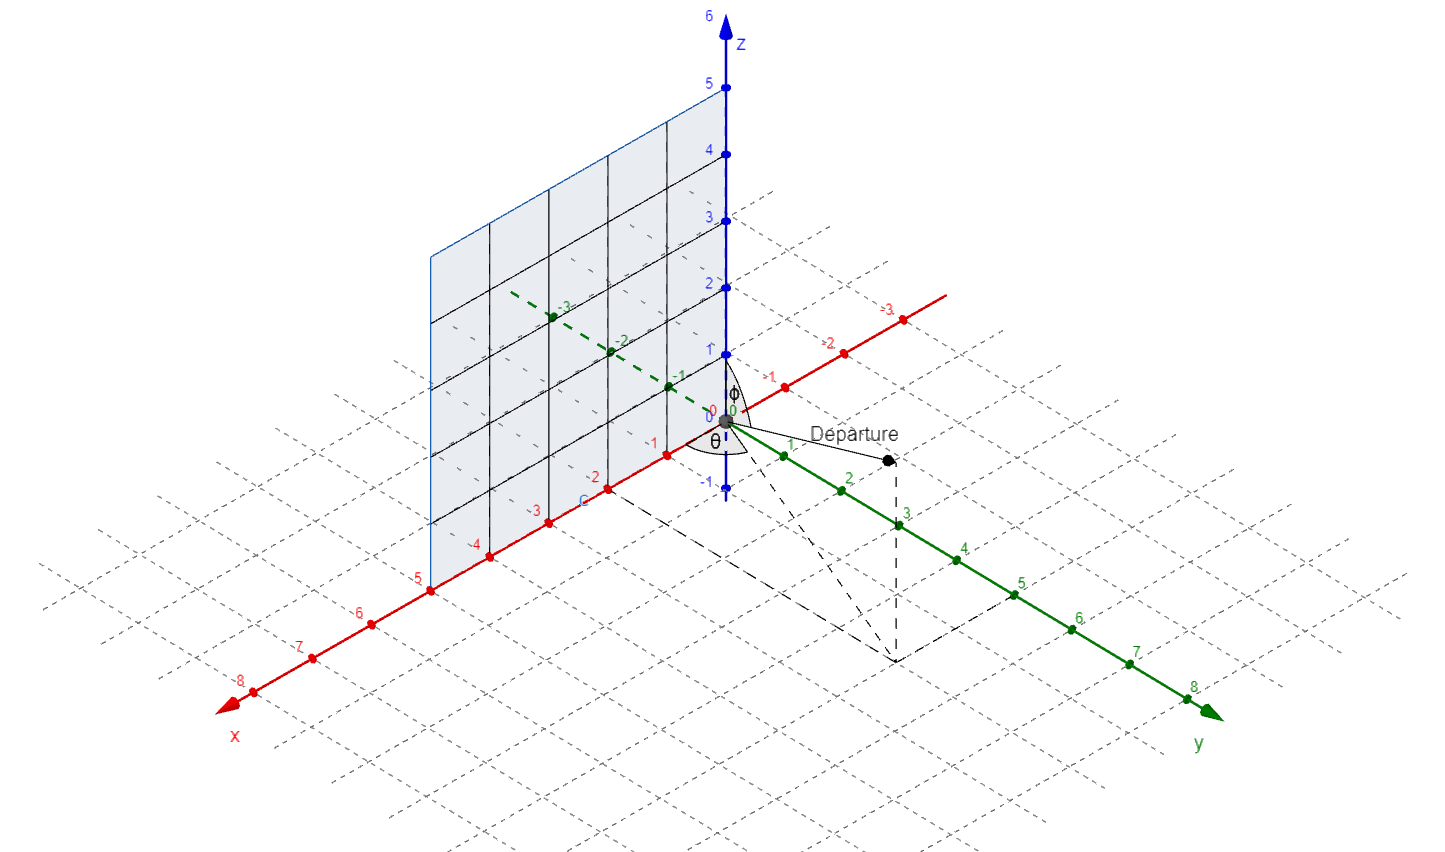
\includegraphics[width=6in]{channelillus.png} 
\caption{Angle of departure} \label{fig:sphangle}
\end{figure}

W.l.o.g., in the following context, the \ac{irs} is placed in the first quadrant of the $xz$-pane. We also assume that $\sqrt M$ is a positive integer. Moreover, we assume that the distances between any two neighboring \ac{irs} elements are constant and are denoted as $d$. The \ac{irs} elements are indexed from right to left (along $x$-axis, $0$ to $+\infty$), bottom to top (along $z$-axis, $0$ to $+\infty$). Based on these conventions, if $m\in \mathbb N \cap [1, M]$, the $m$-th \ac{irs} element will have the coordinate 
\begin{equation}
\begin{bmatrix}
&x=((m-1) \mathrm{mod} \sqrt M)\cdot d, \\
&y=0, \\
&z=\lfloor(m-1)/\sqrt M\rfloor \cdot d
\end{bmatrix}.
\label{eq:coodinateofthemthelem}
\end{equation}
The $\mathrm{mod}$ operator in the above equation is the modulo operation which is evaluated to the remainder of the division of $(m-1)$ by $\sqrt M$. 
The lower half bracket $\lfloor\cdot\rfloor$ is the floor operator that evaluates to the largest interger that is smaller or equal to the number inside it.


The steering vector $\mathbf h_{\mathrm t}^{\mathsf{T}}(\theta_p^{\mathsf{T}}, \phi_p^{\mathsf{T}})$ is described by
\begin{equation}
\mathbf h_{\mathrm t}(\theta_p^{\mathsf{T}}, \phi_p^{\mathsf{T}})=\begin{bmatrix}
e^{j\frac{2\pi d}{\lambda_{\mathrm w}}[((m-1) \mathrm{mod} \sqrt M)\sin(\phi_p^{\mathsf{T}})\cos(\theta_p^{\mathsf{T}})+\lfloor(m-1)/\sqrt M\rfloor\cos(\phi_p^{\mathsf{T}})]}
\end{bmatrix}_{m,1},
\end{equation}
where $\lambda_{\mathrm w}$ denotes the wavelength of the transmitted signal.

In Eq. (\ref{eq:fullchanneldes}), the path loss and the fading is included in the coefficient $h_p$. According to \cite{jamali2020intelligent}, $h_p$ is modeled as $h_p=\sqrt{\bar h_k}\tilde h_p$, where $\bar h_k$ is the path loss of the $k$-th \ac{ut} and $\tilde h_p$ is the random fading of the $p$-th path. Their mathematical descriptions are given by
\begin{equation}
\begin{split}
&\bar h_k=\left(\frac{\lambda_{\mathrm w}}{4\pi l_{\mathrm{ref}}}\right)^n\\
&\tilde h_p\sim\mathrm{CN}(0, \sigma_f^2).
\end{split}
\end{equation}
The variable $n\in \mathbb R$ is the path loss exponent and it is greater or equal than two.  

\subsection{Simulation Setup}
In order to simulate the channel correlations, we place $8$ \acp{ut} at the range of $50+14\times k$ meters, where $k\in\{0,\dots, 7\}$. Each \ac{bs}-\ac{ut} channel consists of $8$ effective paths. The intended messages for the \acp{ut} have the same power $\sigma_s^2=1$. The angles from the \ac{bs} to the scatterings are constant during the whole transmission. 

Since block fading is assumed, the fading parameters are generated once every block. To make the further discussion easier, we assume that the distances between the \acp{ut} and the \ac{bs} are deterministic and known by all the \acp{ut} and the \ac{bs}.
The default settings for the channel are concluded as Table (\ref{table:parametersforthechannel}).
\begin{table}
\begin{tabularx} {1\textwidth}{ 
  | >{\centering\arraybackslash}X 
  | >{\centering\arraybackslash}X 
  | >{\centering\arraybackslash}X
  | >{\centering\arraybackslash}X 
  | >{\centering\arraybackslash}X
  | >{\centering\arraybackslash}X
  | >{\centering\arraybackslash}X
  | >{\centering\arraybackslash}X
  | >{\centering\arraybackslash}X | }
 \hline
 $l_{\mathrm{ref}}$		& $\lambda_{\mathrm{w}}$ 	& $\sigma_f^2$	& $\theta_p^{\mathrm t}, \phi_p^{\mathrm t}$	&$d$& $n$& $P$ & $K$\\
 \hline
 $[50, 150]$	& $0.01$ 			& $1$ 				&$[0, \pi]$ 					&$\lambda_{\mathrm{w}}/2$&$3$& $8$ & $8$\\
\hline
\end{tabularx}
\caption{Parameters for channel $\mathbf H$}
\label{table:parametersforthechannel}
\end{table}

The matrix $\mathbf T$ describes the illumination channel from the active antennas to the \ac{irs} as is defined in Eq.(\ref{eq:illuminationbasic}).
In the simulations, $N$ horn-shape active antennas are uniformly placed on a circle parallel to the $xz$-pane. 
The center of the the active antenna arrays and the center of the \ac{irs} form a line that is also parallel to the $y$-axis.
The radius of the active antenna arrays is denoted as $R_{\mathrm r}$, and the distance between this antenna array and the $xz$-pane is denoted as $R_{\mathrm d}$. 
This array setup is exemplified in Fig. (\ref{fig:activeantepos}).
To investigate the effect of interference on the IRS, two illumination strategies based on the orientations of active antennas are used. 

\begin{figure}[htbp]
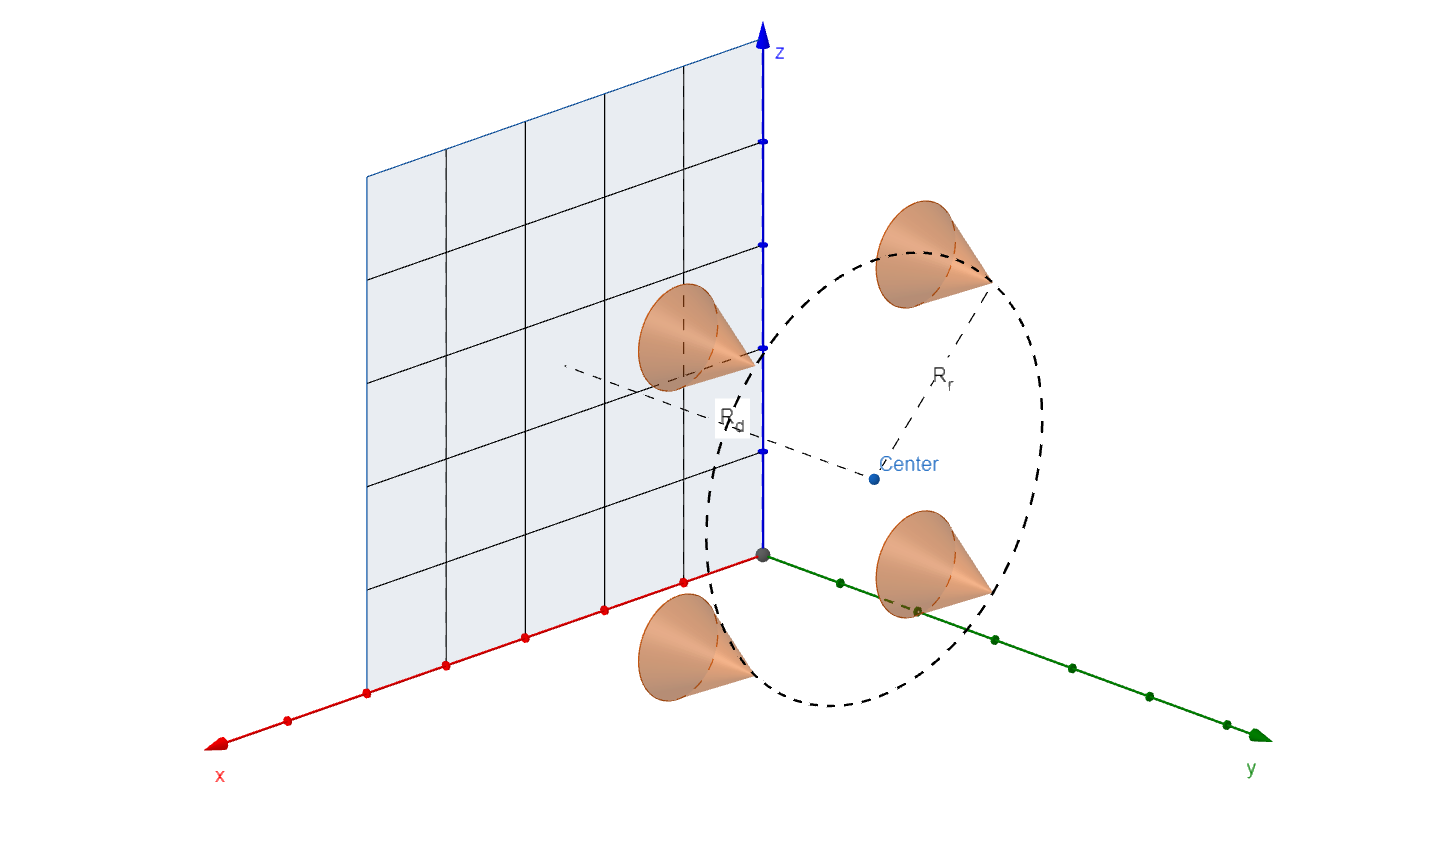
\includegraphics[width=5in]{posantenna.png} 
\caption{Placement of the active antennas} \label{fig:activeantepos}
\end{figure}
%\begin{equation}
%\mathbf T=\begin{bmatrix}
%\frac{\lambda_{\mathrm w}\sqrt{\rho G^{\mathrm a}(\theta^{\mathrm p}_{m,n}, \phi^{\mathrm p}_{m,n})G^{\mathrm p}(\theta^{\mathrm a}_{m,n}, \phi^{\mathrm a}_{m,n})}}{4\pi r_{m,n}}e^{-j\frac{2\pi r_{m,n}}{\lambda_{\mathrm w}}}
%\end{bmatrix}_{m,n},
%\label{eq:illuminationbasic}
%\end{equation}
%where $\rho\in[0,1]$ denotes the power efficiency of the \ac{irs}. The function $G^{\mathrm a}(\theta^{\mathrm p}_{m,n}, \phi^{\mathrm p}_{m,n})$ and $G^{\mathrm p}(\theta^{\mathrm a}_{m,n}, \phi^{\mathrm a}_{m,n})$ model the antenna gain of the active antenna and the \ac{irs} element respectively. The variable $r_{m,n}$ measures the distance from the $m$-th IRS element to the $n$-th active antenna.
%
%
%We assume here that the IRS elements reflect all the signals in front of them, therefore we have 
%\begin{equation}
%G^{\mathrm p}(\theta, \phi)=\begin{cases}
%2 & \theta, \phi\in[0,\pi] \\
%0 & \, \text{otherwise}
%\end{cases}.
%\end{equation}
%
%The active antenna gain following \cite{jamali2020intelligent} is assumed to be 
%\begin{equation}
%G^{\mathrm a}(\theta, \phi)=\begin{cases}
%2(1+\kappa)\cos^\kappa(\phi) & \phi\in[0,\pi/2] \\
%0 & \, \text{otherwise}
%\end{cases}.
%\end{equation}
%The $\kappa$ here is a normalization factor which ensures that the spherical surface integral of $G^{\mathrm a}(\theta, \phi)$ is $4\pi$. With larger $\kappa$, the beam from the active antenna will be more concentrated to its main direction.
%
%Besides the antenna patterns, the orientations of the active antennas also matter. 


In \ac{fi}, all active antenna illuminates toward the center of \ac{irs}. In this way, the IRS receives the most power as well as most interference. This illumination strategy is shown in Fig. (\ref{fig:fi}).
\begin{figure}[htbp]
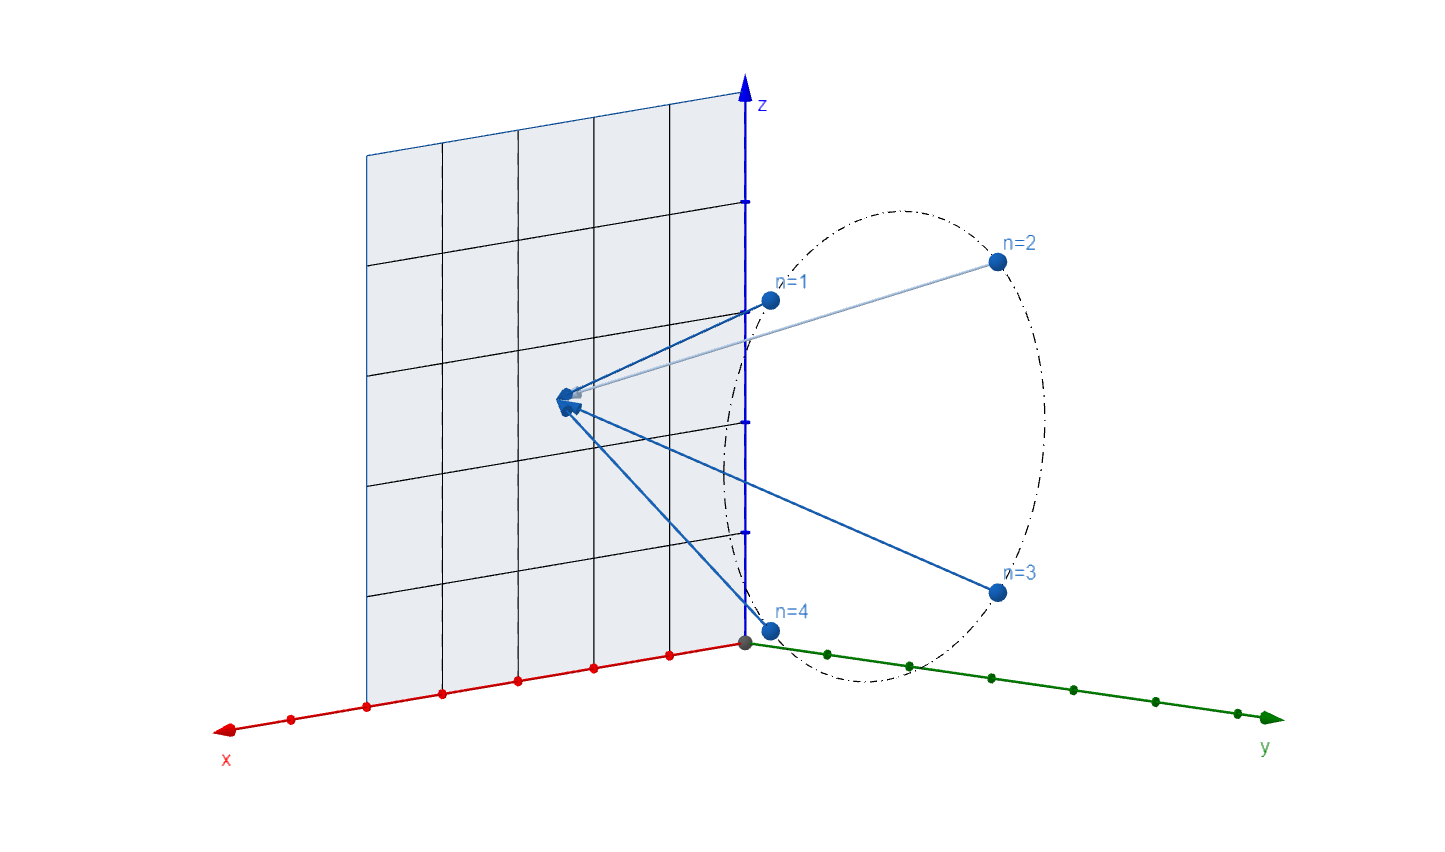
\includegraphics[width=6in]{fullillumination.png} 
\caption{Full illumination} \label{fig:fi}
\end{figure}

In \ac{pi}, we designate $N$ sections on the \ac{irs}, such that each section is responsible for one active antenna. Each active antenna illuminates the signals to the center of its designated section. Fig. (\ref{fig:pi}) depicts this scenario.
\begin{figure}[htbp]
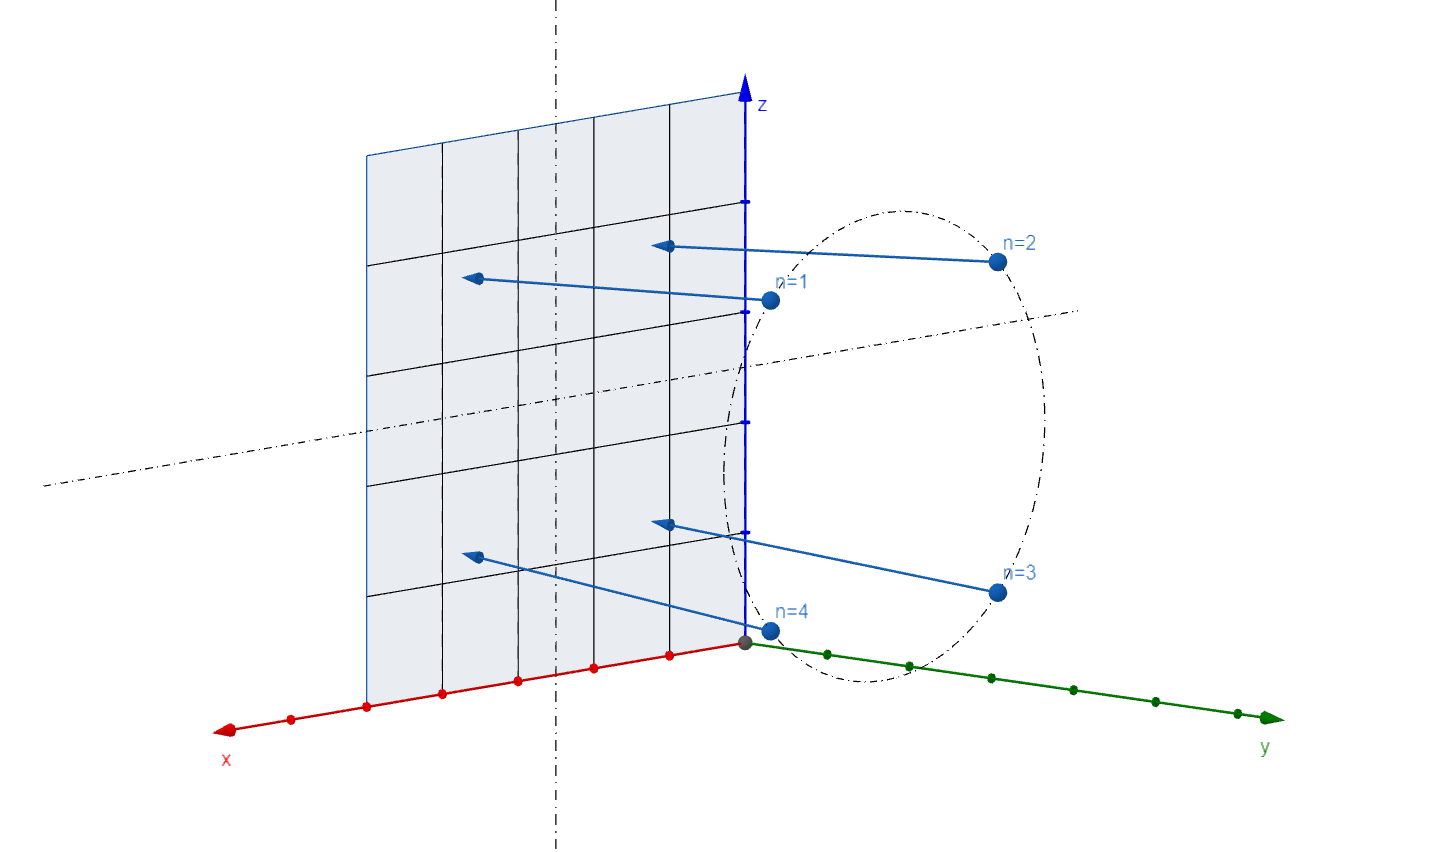
\includegraphics[width=6in]{partialillumination.png} 
\caption{Partial illumination} \label{fig:pi}
\end{figure}

The illumination parameters are concluded in Table (\ref{table:illuminationchannel}) \cite{jamali2020intelligent}.
\begin{table}
\begin{tabularx} {1\textwidth}{ 
  | >{\centering\arraybackslash}X 
  | >{\centering\arraybackslash}X 
  | >{\centering\arraybackslash}X
  | >{\centering\arraybackslash}X 
  | >{\centering\arraybackslash}X
  | >{\centering\arraybackslash}X | }
 \hline
 $\rho$		& $R_{\mathrm d}$	& $R_{\mathrm r}$	& $\kappa$	\\
 \hline
 $1$	& $\mathrm S1:\frac{4d\sqrt{M}}{\sqrt{\pi}}, \mathrm S2:\frac{4d\sqrt{M}}{\sqrt{N\pi}}$ 			& $\mathrm S1:2d, \mathrm S2:\frac{d\sqrt{2M}}{4}$ 				&$49$ 	\\
\hline
\end{tabularx}
\caption{Parameters for fading and path loss}
\label{table:illuminationchannel}
\end{table}




\subsection{Rate and PAPR}
By using the above mentioned setup, and setting IRS antenna element amount to 64, we plot the rate performance for full illumination with gradient descent and MM algorithm. Partial illumination based on MM algorithm is also simulated for comparison. It is assume here that the estimation error is zero and the maximal normalized noise is set to be $\sigma^2_{\tilde n_{\mathrm{max}}}=0.001$ such that it has a similar scale as the interference power. The PAPR is adjusted by increasing the peak power constraint while the regularizer $\lambda$ is fixed to be $0.5$. For block length $L=1$, the result is shown as Fig. (\ref{fig:paprL1}).
\begin{figure}[htbp]\flushleft
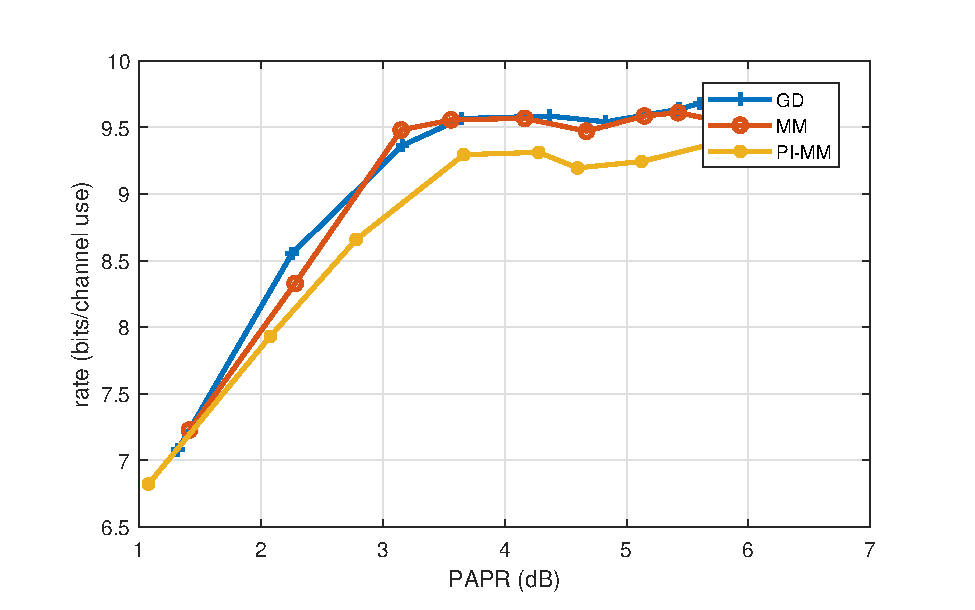
\includegraphics[width=6in]{L1n-3.eps} 
\caption{Rate-PAPR with block length $L=1$, guard interval $\tau=0$ and regularizer $\lambda=0.5$} \label{fig:paprL1}
\end{figure}

It can be observed by comparing the red line and the yellow line that partial illumination strategy performs slightly worse than the full illumination strategy. One reason is the spillover effect caused by the antenna pattern. In full illumination, the IRS receives more power than the partial illumination
strategy. In fact, it can be proven that given enough power and enough IRS size, symbol-wise distortion-free transmission is always achievable.

\begin{theorem}
If \(\mathbf H\) is a complex normal Gaussian random matrix with independent entries and the length of the uni-modular vector \(\mathbf d\) can be arbitrary long, then it is almost certain that there is a \(\mathbf d\) such that \(\mathbf H\cdot\mathbf d=\mathbf 0\).
\label{th:firsttheorem}
\end{theorem}
\begin{proof}
See appendix.
\end{proof}


For the precoding optimization problem with block length $L=1$ and number of RF chains $N=1$. Define $\mathbf H'=\mathbf H\times \mathrm{diag}_\mathrm{matrix}\{x\mathbf t\}$, and the problem is transformed to finding vector $\mathbf d=\mathrm{diag}_{\mathrm{vector}}\{\mathbf A\}$ such that $\mathbf s=\mathbf H'\mathbf d$. To use the theorem, define
\begin{equation}
\begin{split}
\mathbf H''=\begin{bmatrix}
\mathbf H', &\mathbf s
\end{bmatrix}\\
\mathbf d'=\begin{bmatrix}
\mathbf d_{\mathrm{aux}}\\
d_{M+1}
\end{bmatrix}.
\end{split}
\end{equation}
According the the theorem above, a solution for $\mathbf d'$ can be found such that $\mathbf 0=\mathbf H''\mathbf d'$. Therefore the IRS parameters should be $\mathbf A=\mathrm{diag}_{\mathrm{matrix}}\{-d_{M+1}^{-1}\mathbf d_{\mathrm{aux}}\}$. For the cases where more RF chains are used $N>1$, we can always transform it back to the case where $N=1$ by muting all the RF chains except the first one. 


For increased block length, where $L=2$, the simulation results are shown in Fig. (\ref{fig:paprL2}).
\begin{figure}[htbp]\flushleft
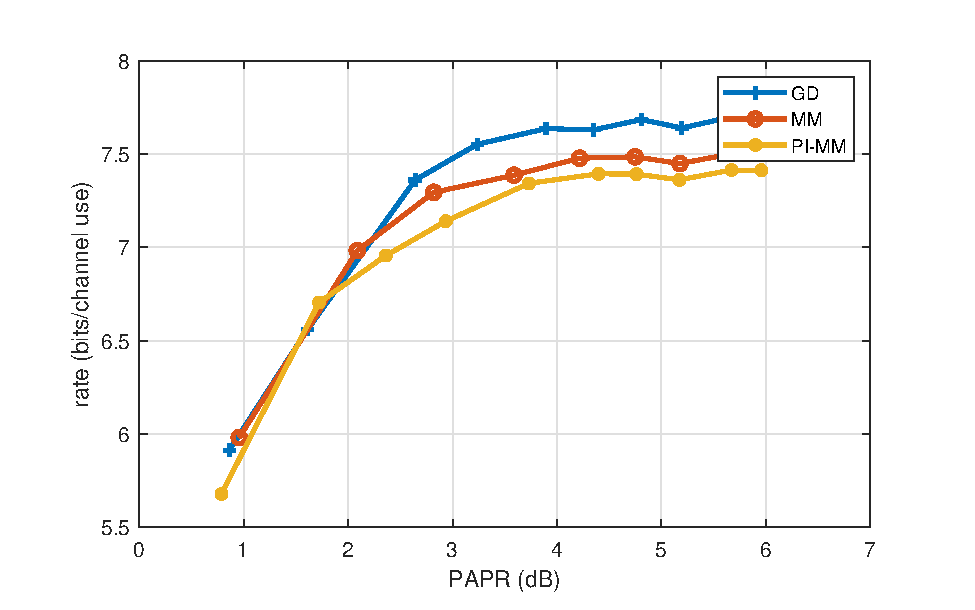
\includegraphics[width=6in]{L2n-3.eps} 
\caption{Rate-PAPR with block length $L=2$, guard interval $\tau=0$ and regularizer $\lambda=0.5$} \label{fig:paprL2}
\end{figure}

It can be seen here that with guard interval $\tau=0$, the systems with larger block lengths tend to have worse rate performance compared to the systems with smaller block lengths. This can be explained by code space density at the receivers side. Let's assume a fixed stream of code and messages with length $L_\mathrm{tot}$. If we have two options for block lengths, $L_1$ and $L_2$. Suppose $L_\mathrm{tot}$ is dividable by $L_1$ and $L_2$.Following Eq. (\ref{eq:decouple}), we can see that the received code at the \acp{ut} side is actually generated by any combination of $(\mathbf x_i, \dots, \mathbf x_{L_\mathrm{tot}}, \mathbf A_i, \dots, \mathbf A_{L_\mathrm{tot}})$ such that  $\mathbf A_i=\mathbf A_j$ if $i$ and $j$ belong to the same time block. There are less constraints for the scheme where smaller block length is used. thus, the system which adopts a smaller block length should have a denser code stream space at the receiver side, and it is more likely for the transmitter to find a code stream that is closer to the intended messages. 


\subsection {Regularizer}
The transmission power is controlled by the regularizer $\lambda$. It balances the emphasis between the interference power and the RF chains signal power. 

In order to study the behavior of regularizer, we set the peak power constraint to infinity and plot the rate-$\lambda$ curves in Fig. (\ref{fig:ratelambda}). The default illumination strategy is \ac{fi}. And the channel estimation error is not included. 

\begin{figure}[htbp]\flushleft
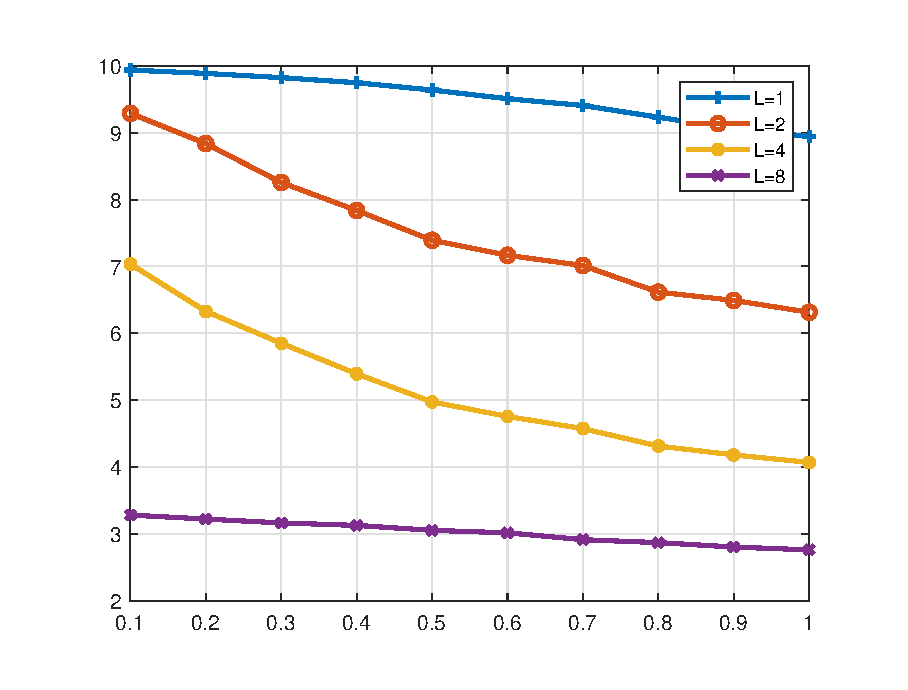
\includegraphics[width=6in]{lmd.eps} 
\caption{Rate-$\lambda$ behavior of MM-algorithm with guard interval $\tau=0$} \label{fig:ratelambda}
\end{figure}

Since $\sigma_{\mathrm{s}}^2=1$ and $\sigma_{\tilde{\mathrm n}_{\mathrm{max}}}^2=0.001$,
 we would have $rate=\log_2 1001\approx9.97$ if the distortion power is zero. Fig. (\ref{fig:ratelambda}) shows that for $L=1$, the curve approaches this rate limit as $\lambda$ tend to zero. This matches the Theorem (\ref{th:firsttheorem}) discussed above.  Similar phenomenon was researched in \cite{sedaghat2017novel}. It states that for full rank $\mathbf H$ and $\mathbf S$, the interference power $\left|\left|\mathbf{H}\mathbf{F}_\mathrm{GA}\mathbf X-\mathbf S\right|\right|_\mathrm{F}^2$ can never be made exactly to zero if the block length is larger than the number of RF chains. The matrix $\mathbf F_{\mathrm{GA}}\in \mathbb C^{M\times N}$ in the statement represents the fully connected analog unit and it can be any complex matrix of size $M\times N$. Since the IRS structure is a special case of general HAD system, this statement can also be used to explain the purple curve standing for $L=8$. However, it is also stated in \cite{sedaghat2017novel} that if the block length is smaller than the RF chain number,  the distortion in a fully connected transmission system can always be made to zero. Since the optimization method we use here is sub-optimal, the validity of this proposition in IRS-aided transmission systems remains unknown.


The relation between the average RF chain power and the regularizer lambda is shown as Fig. (\ref{fig:powerlambda}).
\begin{figure}[htbp]\flushleft
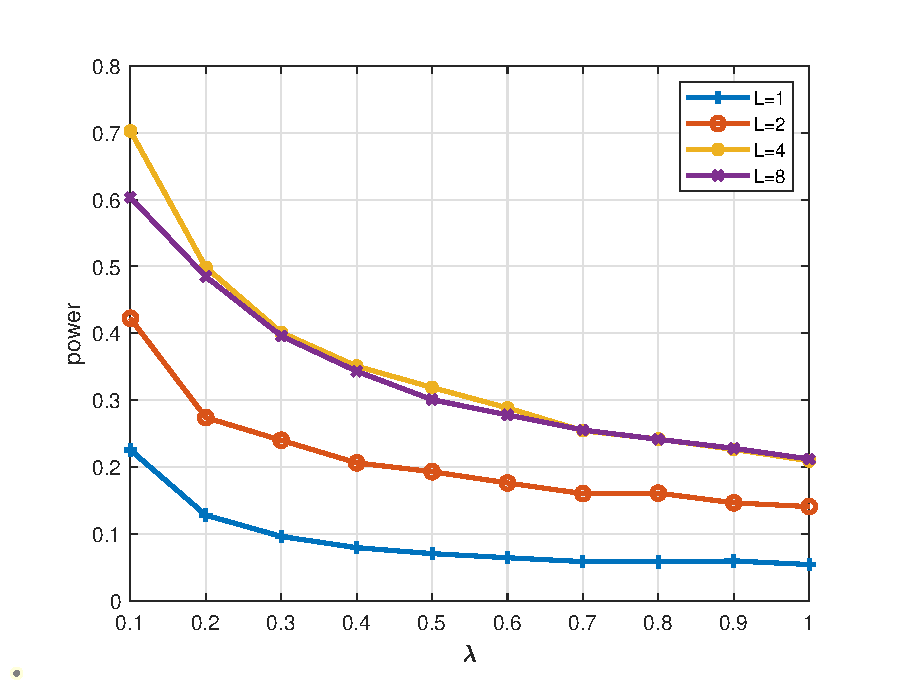
\includegraphics[width=6in]{lmdpower.eps} 
\caption{Average RF chain power-$\lambda$ with guard interval $\tau=0$} \label{fig:powerlambda}
\end{figure}
For relative small block lengths, the system with small $L$ performs better. However, for systems with relative large block lengths, the power curves are close to each other. The reason for this can be explained by analyzing the objective function. 

For smaller block lengths, the interference power can be made very small. As a result, the dominant part of the objective function is the term for transmission power. Thus, the system with small $L$ will put more emphasis on reducing the RF chain power. However, systems with larger $L$ will concentrate on minimizing the interference power. 

\subsection{Rate, Block Length and Number of IRS Elements}
Now, set the guard interval to $\tau=T_{\mathrm{s}}$ and remove the peak power constraint. We assumes that the normalized channel estimation error matrix is comprised of i.i.d. entries \cite{zetterberg2011experimental}, i.e. 
\begin{equation}
\begin{split}
\forall k\in\mathbb N\cap[1, K], \sigma_{\mathrm{e},{k}}^2/\bar{h}_k=\sigma_{\tilde{\mathrm e}}^2,
\end{split}
\end{equation}
where $\sigma_{\tilde{\mathrm e}}^2$ is the variance of the entries of the normalized estimation error matrix.

 The Fig. (\ref{fig:rateML10}) shows that the achievable rate increases as the number of IRS elements increases and the rate decreases as the variance of the estimation error increases, which are expected.
\begin{figure}[!htb]\flushleft
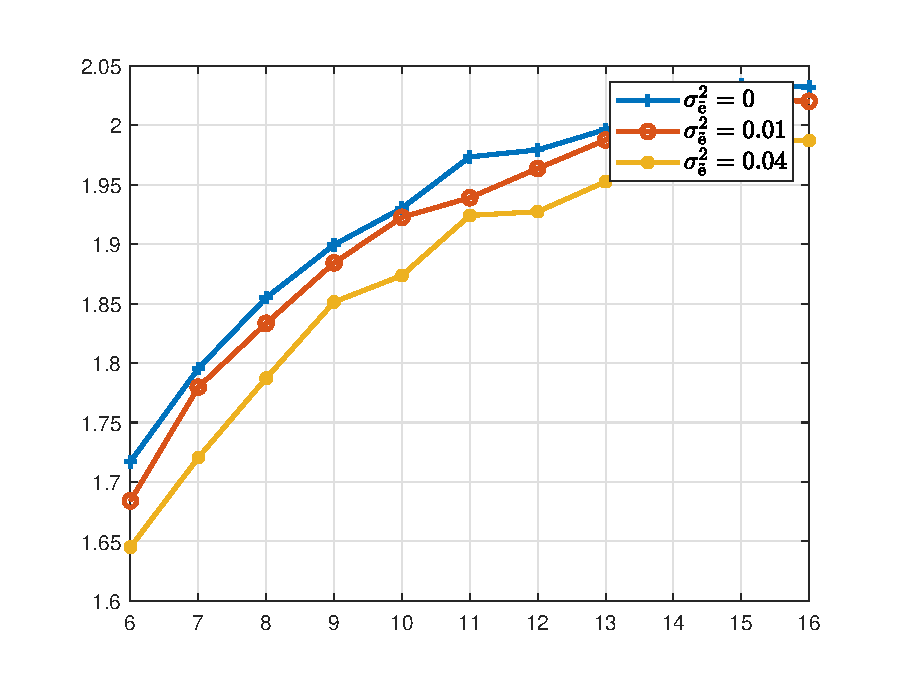
\includegraphics[width=6in]{rate-surdM.eps} 
\caption{Rate-$\sqrt M$ with guard interval $\tau=T_{\mathrm{s}}$ and $L=10$} \label{fig:rateML10}
\end{figure}

Next, we want to study the rate-block length behavior. The number of IRS elements is set to $M=144$, and the simulation results are plotted in Fig. (\ref{fig:rateLM12}).
\begin{figure}[!htb]\flushleft
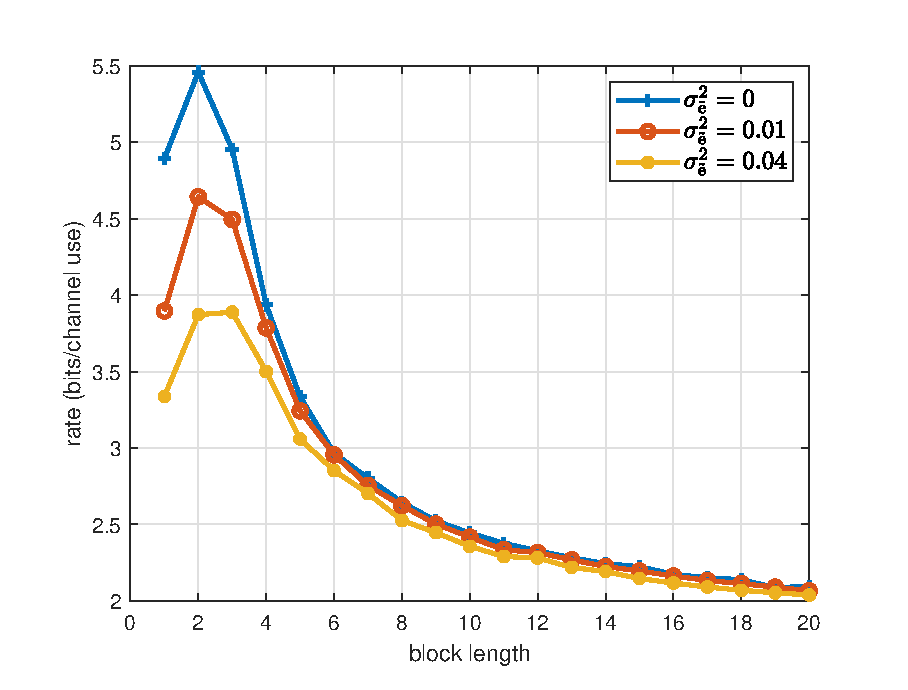
\includegraphics[width=6in]{Rate_Lwithm12.eps} 
\caption{Rate-$L$ with guard interval $\tau=T_{\mathrm{s}}$ and $M=144$} \label{fig:rateLM12}
\end{figure}
In this figure, the rate first increases and then decreases. This phenomenon is caused by the non-zero guard interval.

 For smaller block length, the interference is small relative to the noise power. As a result, the dominant part is the guard interval. It can be seen that the at $L=1$ the rate of the estimation error free curve is $4.9 (\mathrm{bits/channel use})$ which is close to one half of $\log_21001$. This is consistent with Theorem (\ref{th:firsttheorem}). As the block length increases, the term $\frac{LT_{\mathrm{s}}}{\tau+LT_{\mathrm{s}}}$ tends to $1$ and the dominant part becomes the term $\log(1+SINR)$. 

Based on these two points, we can predict that for larger $\tau$, the peak of the rate-L plot will shift to right since the term $\frac{LT_{\mathrm{s}}}{\tau+LT_{\mathrm{s}}}$ monotonically increases as $L$ increases while the term $\log(1+SINR)$ decreases as $L$ increases. The complete relation of rate, $\sqrt M$ and $L$ are shown as a mesh surface in Fig. (\ref{fig:fullrelation3d}).
\begin{figure}[htbp]
 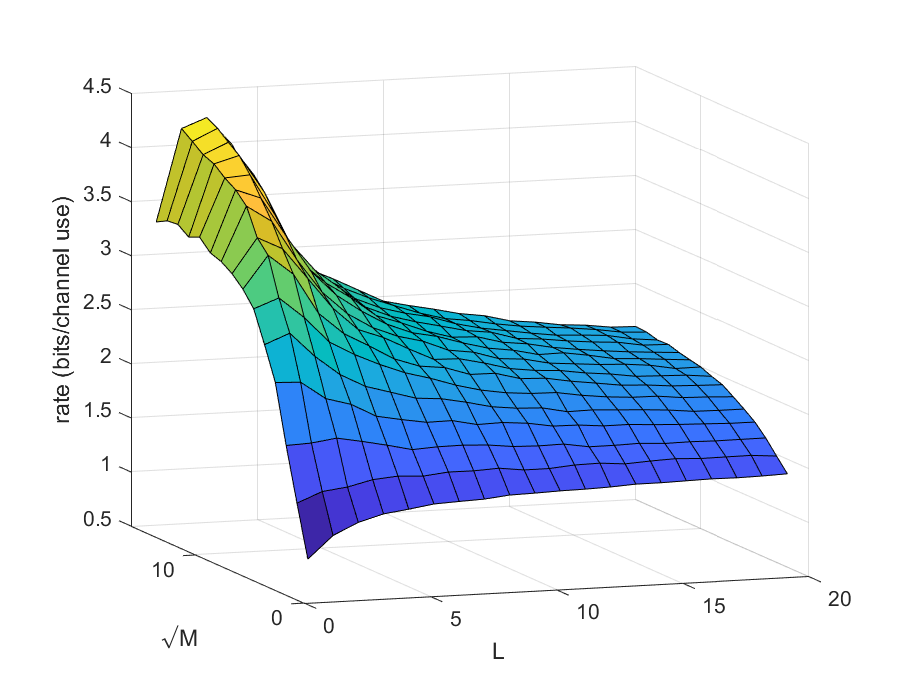
\includegraphics[width=6in]{threed.eps}
  \caption{Impact of IRS size and Block size ($\tau=1$)}
  \label{fig:fullrelation3d}
\end{figure}

At last it would also be interesting to know the minimal required IRS elements to achieve a certain rate with increasing block length. Instead of directly plotting by reading Fig. (\ref{fig:fullrelation3d}), we calculate the rate of each transmission block, and use this value to obtain the averaged minimal IRS size for reaching a certain rate. 

For rate threshold $2.1\mathrm{(bits/channel use)}$, the averaged minimal $M$ versus $L$ is plotted as Fig. (\ref{fig:MLr18}). 
\begin{figure}[htbp]\flushleft
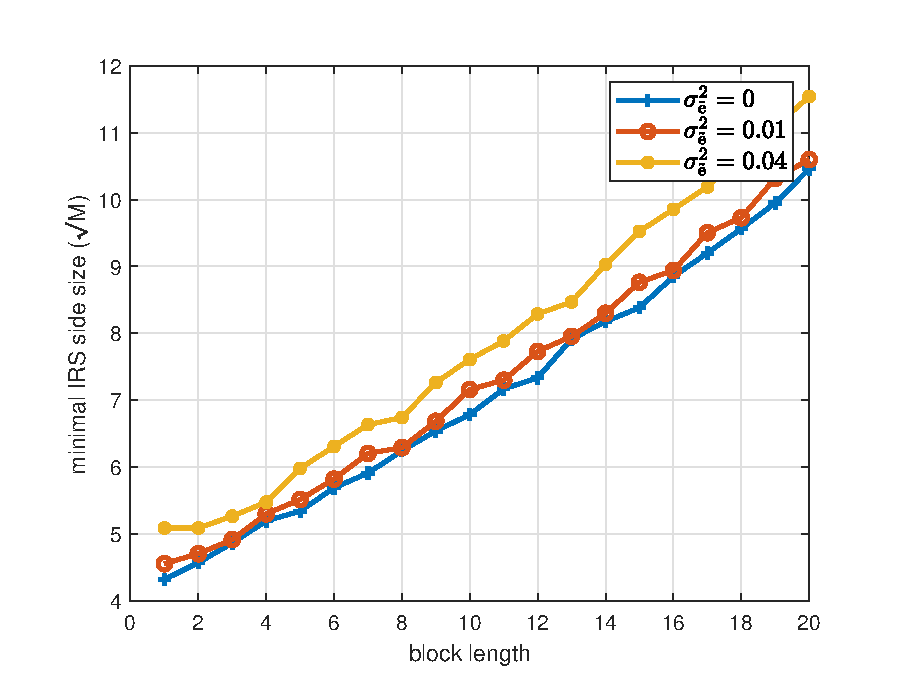
\includegraphics[width=6in]{requiredSurdM.eps} 
\caption{Averaged minimal $M$-$L$ with rate\_threshold$=1.8$} \label{fig:MLr18}
\end{figure}
It shows that the minimal required IRS size has an approximately quadratical growth rate as the block length if the threshold rate is achievable. This means we can trade the IRS update rate with IRS size efficiently. However, if both higher data rate and lower update rate are desired, we may have to increase the number of RF chains as is suggested in \cite{sedaghat2017novel}.


\section{Appendix}
\subsection{Proof for Theorem 1}
For the simple case where $\mathbf H$ is a row vector, namely when there is only one user $K=1$,  define $\mathbf h^{\mathsf{T}}=\mathbf H$. We then try to find out the lower bound of probability $\mathrm{Pr}(\exists \mathbf d,(\mathbf h^{\mathsf{T}} \mathbf d=0))$. 

This can be translated into geometry representations. Each complex entry in vector $\mathbf h^{\mathsf{T}}$ is an 2-D vector whose length is a random variable following standard Gaussian distribution and phase is uniformly distributed between $0$ to $2\pi$. From this point of view, the uni-modular vector $\mathbf d$ represents the rotation operations which are applied to the columns of $\mathbf h^{\mathsf{T}}$ with controllable angles. Therefore, the proposition $\exists \mathbf d,(\mathbf h^{\mathsf{T}} \mathbf d=0)$ can be interpreted as finding an rotation angle for each of the entries in vector $\mathbf h^{\mathsf{T}}$ such that these rotated entries add up to zero. Following triangular inequality, we can say that there exists a vector $\mathbf d$, such that $\mathbf h^{\mathsf{T}} \mathbf d=0$. This means
\begin{equation}
\begin{split}
\max(|h_1|, \dots, |h_M|)\leq|h_1|+\dots+|h_M|-\max(|h_1|, \dots, |h_M|).
\end{split}
\end{equation}
It can also be observed that $|h_1|>|h_2|+\dots+|h_M|$ and  $|h_2|>|h_1|+\dots+|h_M|$ will never happen simultaneously. Therefore, we can write the above probability in negation form while taking the independence assumption into consideration
 \begin{equation}
\begin{split}
P_1=&\mathrm{Pr}(\exists \mathbf d,(\mathbf h^{\mathsf{T}} \mathbf d=0))\\
=&1-(M\times \mathrm{Pr}(|h_1|>|h_2|+\dots+|h_M|))
\end{split}
\end{equation}
The properties of F-distribution can be used to determine the upper bound of $\mathrm{Pr}(|h_1|>|h_2|+\dots+|h_M|)$.
\begin{equation}
\begin{split}
&M\times \mathrm{Pr}(|X|>|X_1|+\dots+|X_{M-1}|)\\
\leq &M\times \mathrm{Pr}(|X|^2>|X_1|^2+\dots+|X_{M-1}|^2)\\
\leq &M\times \mathrm{Pr}(|X|^2+|Y|^2>|X_1|^2+\dots+|X_{M-1}|^2)\\
= &M\times \mathrm{Pr}\left(\frac{2}{M-1}>\frac{(|X_1|^2+\dots+|X_{M-1}|^2)/(M-1)}{(|X|^2+|Y|^2)/2}\right)\\
=&M\times F\left(\frac{2}{M-1}; M-1, 2\right)=M\times I_{\frac{1}{2}}\left(\frac{M-1}{2}, 1\right)\\
=&M\times \left(\frac{1}{2}\right)^{\frac{M-1}{2}},
\end{split}
\end{equation}
where $F(x; z_1, z_2)$ is the cumulative distribution function with $z_1$ and $z_2$ degrees of freedom and $I_x(a,b)$ is the regularized incomplete beta function.
The first less equal sign holds because $|X|^2>(|X_1|^2+\dots+|X_{M-1}|^2)^2>|X_1|^2+\dots+|X_{M-1}|^2$.

 For the multi-user case where $K\neq 1$, the matrix $\mathbf H$ has more than one rows. A solution for $\mathbf d$ can be constructed recursively. 

We first try to construct a sufficient condition for the existence of such vector $\mathbf d$. Then we try to prove that the probability for this sufficient condition not to hold tends to zero. 

For sake of simplicity, we denote the channel matrix as $\mathbf H^{(k)}$ if $K=k$. Suppose we know how to construct $\mathbf d$ if $K=k-1$ such that $\mathbf H^{(k-1)}\cdot \mathbf d=\mathbf 0$. This also implies that $(\mathbf H^{(k-1)}\cdot \mathbf d)\cdot e^{j\varphi}=\mathbf 0$, where $\varphi$ is an arbitary number.
 
  Based on these assumptions and discussions, for the case where $K=k$, we can sectorize $\mathbf H^{(k)}$ as Fig. (\ref{fig:idea}) and sectorize $\mathbf d$ into several vecrtors correspondingly.
\begin{figure}
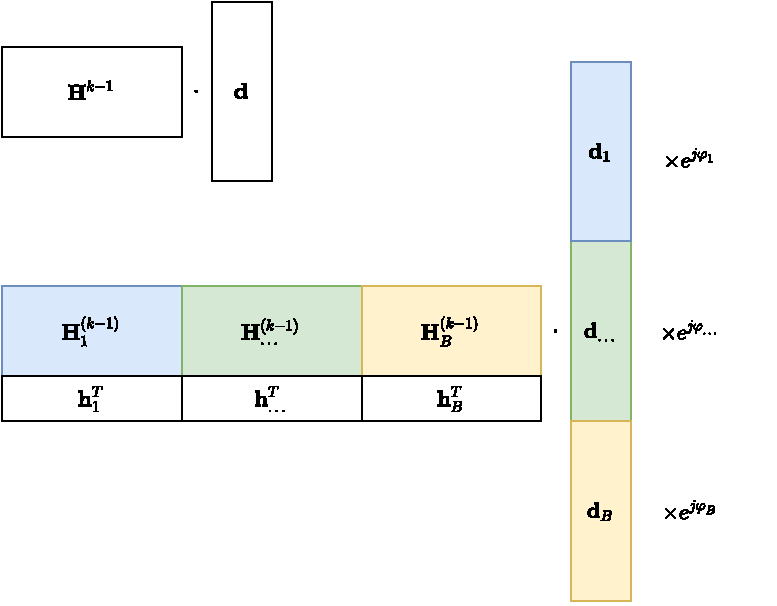
\includegraphics[width=5in]{ideaofproof.pdf} 
\caption{Idea of construction}
\label{fig:idea}
\end{figure}


We only need to find one solution for this problem, and the condition for that solution to exist can serve as sufficient condition for $\exists \mathbf d,(\mathbf H^{(k)} \mathbf d=0)$. 

One instance of $\mathbf d$ may be constructed via the following steps. We first find $\mathbf d_1, \dots, \mathbf d_B$ such that $\forall i\in\{1,\dots, B\},\mathbf H^{(k-1)}_i\mathbf d_i=\mathbf 0$. Then for the last row of matrix $\mathbf H^{(k)}$, we know that $\mathbf h_i^T\cdot \mathbf d_i$ is a scalar value. At the same time, for each subvector $\mathbf d_i$, we can still apply an additional rotation $e^{j\varphi_i}$ to each of the vectors $\mathbf d_i$.

Now the problem is transformed back to the simple case, where we want to find rotation angles $\varphi_1,\dots,\varphi_B$ such that
\begin{equation}
\begin{bmatrix}
\mathbf h_1^{\mathsf{T}}\mathbf d_1 &\dots &\mathbf h_B^{\mathsf{T}}\mathbf d_B
\end{bmatrix}\cdot\begin{bmatrix}
 e^{j\varphi_1}\\
 \vdots\\
e^{j\varphi_B}
\end{bmatrix}=0
\end{equation}
By finding appropriate $\mathbf d_i$ and $\varphi_i$, the rotation vector $\mathbf d$ is obtained.
This is the general idea for the proof. Next, we will provide a detailed proof for this theorem.

Suppose $\mathbf H^{(k)}$ has $M$ columns. We can find at least one $E\in\mathbb N$, such that $M\in[E^k, (E+1)^k]$. We then sectorize the matrix $\mathbf H^{(k)}$ with the scheme shown as Fig. (\ref{fig:constructfinal}). It is worth noticing that the sectorization method is not unique, the only requirement is that the number of columns in each sub-matrix lies within the range of $[E^{k-1}, (E+1)^{k-1}]$. After the sectorization, there are either $E$ or $E+1$ blocks in total.
\begin{figure}
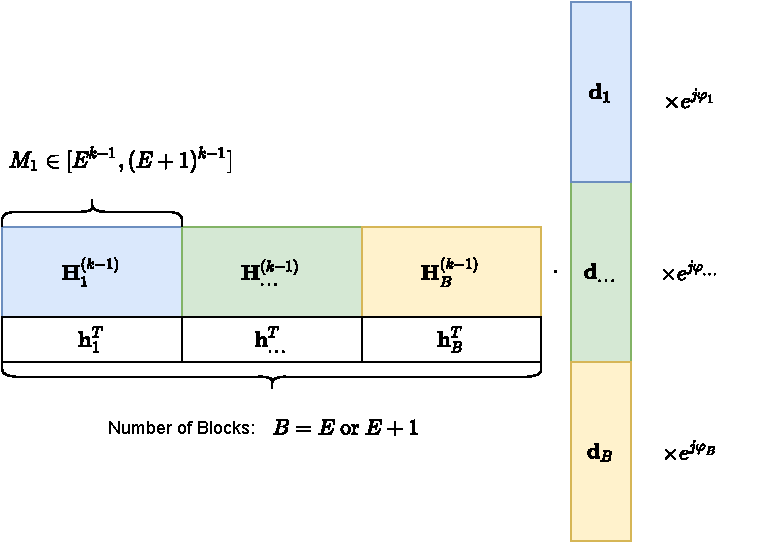
\includegraphics[width=5.5in]{submatrixcons.pdf} 
\caption{Submatrix Construction}
\label{fig:constructfinal}
\end{figure}

If the rotation vector $\mathbf d$ cannot be found with the idea illustrated in Fig (\ref{fig:idea}), then one of the two sufficient conditions does not hold, i.e., either one of the colored submatrix $\mathbf H_i^{(k-1)}$ cannot be rotated to zero or the last row of $\mathbf H^{(k)}$ cannot be made zero. Recursive method can be used to calculate the probability that one of the colored sub-matrices cannot be made zero. We focus on analyzing the last row of matrix $\mathbf H^{(k)}$ first. Define
\begin{equation}
\begin{split}
&B\in\{E, E+1\} : \text{number of blocks}\\
&M_{1\dots B}\in[E^{k-1}, (E+1)^{k-1}]: \text{number of columns in one block}.
\end{split}
\end{equation}
as is also illustrated in Fig. (\ref{fig:constructfinal}). Each block $\mathbf h_i^T$ in the last row will be multiplied with correspondent vector block $\mathbf d_i$,which creates a complex Gaussian random variable $\mathbf h_i^T\mathbf d_i\sim CN(0, M_i)$. The F-distribution is defined on the normal Gaussian variables. Thus, we should first normalize the variance to $1$. This is done in Eq. (\ref{eq:chap5normalizetoF1}) and Eq. (\ref{eq:chap5FdistriMultirow})
Define
\begin{equation}
\begin{split}
&\forall b\in\{1,\dots,B\},Y_b=\mathbf h_b^{\mathsf{T}}\mathbf d_b\sim \mathrm{CN}(0, M_b)\\
&\forall b\in\{1,\dots,B\}, X_b\sim \mathrm{CN}(0, 1).
\label{eq:chap5normalizetoF1}
\end{split}
\end{equation}
Then we have
\begin{equation}
\begin{split}
 &\sum_{b=1}^B \mathrm{Pr}\left(|Y_b|>|Y_1|+\dots+|Y_{b-1}|+|Y_{b+1}|+\dots+|Y_B|\right) \\
\leq &\sum_{b=1}^B \mathrm{Pr}\left(|Y_b|>\sqrt{M_{\mathrm{min}}}\left(\frac {|Y_1|} {\sqrt{M_i}}+\dots+\frac {|Y_{b-1}|}{\sqrt{M_{b-1}}}+\frac{|Y_{b+1}|}{\sqrt{M_{b+1}}}+\dots+\frac{|Y_B|}{\sqrt{M_B}}\right)\right)\\
=&\sum_{b=1}^B \mathrm{Pr}\left(\frac{\sqrt{M_b}}{\sqrt{M_{\mathrm{min}}}}\frac{|Y_b|}{\sqrt{M_b}}>|X_1|+\dots+|X_{B-1}|\right)\\
\leq &B\times \mathrm{Pr}\left(\frac{\sqrt{M_{\mathrm{max}}}}{\sqrt{M_{\mathrm{min}}}}|X|>|X_1|+\dots+|X_{B-1}|\right)\\
\leq &B\times \left( \frac{M_{\mathrm{max}}}{M_{\mathrm{max}}+M_{\mathrm{min}}}\right)^\frac{B-1}{2}.
\label{eq:chap5FdistriMultirow}
\end{split}
\end{equation}
For larger $M$, we have
\begin{equation}
\lim_{M \to +\infty} \frac{M_{\mathrm{max}}}{M_{\mathrm{max}}+M_{\mathrm{min}}}\leq \lim_{E \to +\infty}\frac{(E+1)^{k-1}}{2\times E^{k-1}}=\frac{1}{2}\leq \frac{2}{3}.
\end{equation}
Therefore, 
\begin{equation}
\mathrm{Pr}\left(\nexists (\varphi_1,\cdots, \varphi_B).
\begin{bmatrix}
\mathbf h_1^{\mathsf{T}}\mathbf d_1 &\dots &\mathbf h_B^{\mathsf{T}}\mathbf d_B
\end{bmatrix}\cdot\begin{bmatrix}
 e^{j\varphi_1}\\
 \vdots\\
e^{j\varphi_B}
\end{bmatrix}=0\right)
\leq(N+1)\times \left(\frac 2 3\right)^{\frac{E-1}{2}}.
\end{equation}
The bound for the complete probability can then be obtained
\begin{equation}
\begin{split}
P_k&=\mathrm{Pr}(\nexists \mathbf d,(\mathbf H^{(k)\mathsf{T}} \mathbf d=0))\\
&\leq (E+1)\times P_{k-1}+(E+1)\times \left(\frac 2 3\right)^{\frac{E-1}{2}}.
\end{split}
\end{equation}
Based on this inequality, one can define an auxiliary sequence for the upper bound of the probabilities iteratively
\begin{equation}
\begin{split}
&P_1'=(E+1)\times \left(\frac 2 3\right)^{\frac{E-1}{2}}\\
&P_k'=(E+1)\times P_{k-1}+(E+1)\times \left(\frac 2 3\right)^{\frac{E-1}{2}}.
\end{split}
\end{equation}
By using mathematical induction, it can be proven that $\forall k\in \mathbb N, P_k<P_k'$. This sequence can also be written in analytic form by solving difference equation as
\begin{equation}
P^\prime_k=\frac{(E+1)^{k+1}-(E+1)}{E}\left(\frac{2}{3}\right)^{\frac{E-1}{2}}.
\end{equation}
It can be observed that this upper bound will converge to zero if $E$ tend to infinity.

\begin{acronym}
 \acro{AWGN}{additive white Gaussian noise}
 \acro{SNR}[\ensuremath{\mathrm{SNR}}]{Signal-to-Noise Ratio}
 \acro{mimo}[MIMO]{multiple-input multiple-output}
 \acro{irs}[IRS]{intelligent reflecting surface}
 %\acroplural{irs}[IRSs]{intelligent reflecting surfaces}
 \acro{sinr}[SINR]{signal to noise and interference ratio}
 \acro{had}[HAD]{hybrid analog-digital}
 \acro{csi}[CSI]{channel state information}
 \acro{tdd}[TDD]{time division duplex}
 \acro{rf}[RF]{radio frequency}
 \acro{bs}[BS]{base station}
 \acro{ut}[UT]{user terminal}
 %\acroplural{ut}[UTs]{user terminals}
 \acro{glse}[GLSE]{generalized least-square-error}
 \acro{aoa}[AoA]{angle-of-arrival}
 \acro{aod}[AoD]{angle-of-departure}
 \acro{papr}[PAPR]{peak-to-average-power-ratio}
 \acro{fi}[FI]{full illumination}
 \acro{pi}[PI]{partial illumination}
 \acro{si}[SI]{seperate illumination}
 \acro{rss}[RSS]{residual sum of squares}
 \acro{mm}[MM]{majorize-minimization}
  \acro{iid}[i.i.d.]{independent and identical distribution}
\end{acronym}

\bibliographystyle{IEEEtran}	
\bibliography{Bib}
\end{document}
